\documentclass{ximera}

 

\usepackage{epsfig}

\graphicspath{
  {./}
  {figures/}
}

\usepackage{morewrites}
\makeatletter
\newcommand\subfile[1]{%
\renewcommand{\input}[1]{}%
\begingroup\skip@preamble\otherinput{#1}\endgroup\par\vspace{\topsep}
\let\input\otherinput}
\makeatother

\newcommand{\includeexercises}{\directlua{dofile("/home/jim/linearAlgebra/laode/exercises.lua")}}

%\newcounter{ccounter}
%\setcounter{ccounter}{1}
%\newcommand{\Chapter}[1]{\setcounter{chapter}{\arabic{ccounter}}\chapter{#1}\addtocounter{ccounter}{1}}

%\newcommand{\section}[1]{\section{#1}\setcounter{thm}{0}\setcounter{equation}{0}}

%\renewcommand{\theequation}{\arabic{chapter}.\arabic{section}.\arabic{equation}}
%\renewcommand{\thefigure}{\arabic{chapter}.\arabic{figure}}
%\renewcommand{\thetable}{\arabic{chapter}.\arabic{table}}

%\newcommand{\Sec}[2]{\section{#1}\markright{\arabic{ccounter}.\arabic{section}.#2}\setcounter{equation}{0}\setcounter{thm}{0}\setcounter{figure}{0}}

\newcommand{\Sec}[2]{\section{#1}}

\setcounter{secnumdepth}{2}
%\setcounter{secnumdepth}{1} 

%\newcounter{THM}
%\renewcommand{\theTHM}{\arabic{chapter}.\arabic{section}}

\newcommand{\trademark}{{R\!\!\!\!\!\bigcirc}}
%\newtheorem{exercise}{}

\newcommand{\dfield}{{\sf dfield9}}
\newcommand{\pplane}{{\sf pplane9}}

\newcommand{\EXER}{\section*{Exercises}}%\vspace*{0.2in}\hrule\small\setcounter{exercise}{0}}
\newcommand{\CEXER}{}%\vspace{0.08in}\begin{center}Computer Exercises\end{center}}
\newcommand{\TEXER}{} %\vspace{0.08in}\begin{center}Hand Exercises\end{center}}
\newcommand{\AEXER}{} %\vspace{0.08in}\begin{center}Hand Exercises\end{center}}

% BADBAD: \newcommand{\Bbb}{\bf}

\newcommand{\R}{\mbox{$\Bbb{R}$}}
\newcommand{\C}{\mbox{$\Bbb{C}$}}
\newcommand{\Z}{\mbox{$\Bbb{Z}$}}
\newcommand{\N}{\mbox{$\Bbb{N}$}}
\newcommand{\D}{\mbox{{\bf D}}}
\usepackage{amssymb}
%\newcommand{\qed}{\hfill\mbox{\raggedright$\square$} \vspace{1ex}}
%\newcommand{\proof}{\noindent {\bf Proof:} \hspace{0.1in}}

\newcommand{\setmin}{\;\mbox{--}\;}
\newcommand{\Matlab}{{M\small{AT\-LAB}} }
\newcommand{\Matlabp}{{M\small{AT\-LAB}}}
\newcommand{\computer}{\Matlab Instructions}
\newcommand{\half}{\mbox{$\frac{1}{2}$}}
\newcommand{\compose}{\raisebox{.15ex}{\mbox{{\scriptsize$\circ$}}}}
\newcommand{\AND}{\quad\mbox{and}\quad}
\newcommand{\vect}[2]{\left(\begin{array}{c} #1_1 \\ \vdots \\
 #1_{#2}\end{array}\right)}
\newcommand{\mattwo}[4]{\left(\begin{array}{rr} #1 & #2\\ #3
&#4\end{array}\right)}
\newcommand{\mattwoc}[4]{\left(\begin{array}{cc} #1 & #2\\ #3
&#4\end{array}\right)}
\newcommand{\vectwo}[2]{\left(\begin{array}{r} #1 \\ #2\end{array}\right)}
\newcommand{\vectwoc}[2]{\left(\begin{array}{c} #1 \\ #2\end{array}\right)}

\newcommand{\ignore}[1]{}


\newcommand{\inv}{^{-1}}
\newcommand{\CC}{{\cal C}}
\newcommand{\CCone}{\CC^1}
\newcommand{\Span}{{\rm span}}
\newcommand{\rank}{{\rm rank}}
\newcommand{\trace}{{\rm tr}}
\newcommand{\RE}{{\rm Re}}
\newcommand{\IM}{{\rm Im}}
\newcommand{\nulls}{{\rm null\;space}}

\newcommand{\dps}{\displaystyle}
\newcommand{\arraystart}{\renewcommand{\arraystretch}{1.8}}
\newcommand{\arrayfinish}{\renewcommand{\arraystretch}{1.2}}
\newcommand{\Start}[1]{\vspace{0.08in}\noindent {\bf Section~\ref{#1}}}
\newcommand{\exer}[1]{\noindent {\bf \ref{#1}}}
\newcommand{\ans}{}
\newcommand{\matthree}[9]{\left(\begin{array}{rrr} #1 & #2 & #3 \\ #4 & #5 & #6
\\ #7 & #8 & #9\end{array}\right)}
\newcommand{\cvectwo}[2]{\left(\begin{array}{c} #1 \\ #2\end{array}\right)}
\newcommand{\cmatthree}[9]{\left(\begin{array}{ccc} #1 & #2 & #3 \\ #4 & #5 &
#6 \\ #7 & #8 & #9\end{array}\right)}
\newcommand{\vecthree}[3]{\left(\begin{array}{r} #1 \\ #2 \\
#3\end{array}\right)}
\newcommand{\cvecthree}[3]{\left(\begin{array}{c} #1 \\ #2 \\
#3\end{array}\right)}
\newcommand{\cmattwo}[4]{\left(\begin{array}{cc} #1 & #2\\ #3
&#4\end{array}\right)}

\newcommand{\Matrix}[1]{\ensuremath{\left(\begin{array}{rrrrrrrrrrrrrrrrrr} #1 \end{array}\right)}}

\newcommand{\Matrixc}[1]{\ensuremath{\left(\begin{array}{cccccccccccc} #1 \end{array}\right)}}



\renewcommand{\labelenumi}{\theenumi)}
\newenvironment{enumeratea}%
{\begingroup
 \renewcommand{\theenumi}{\alph{enumi}}
 \renewcommand{\labelenumi}{(\theenumi)}
 \begin{enumerate}}
 {\end{enumerate}\endgroup}



\newcounter{help}
\renewcommand{\thehelp}{\thesection.\arabic{equation}}

%\newenvironment{equation*}%
%{\renewcommand\endequation{\eqno (\theequation)* $$}%
%   \begin{equation}}%
%   {\end{equation}\renewcommand\endequation{\eqno \@eqnnum
%$$\global\@ignoretrue}}

%\input{psfig.tex}

\author{Martin Golubitsky and Michael Dellnitz}

%\newenvironment{matlabEquation}%
%{\renewcommand\endequation{\eqno (\theequation*) $$}%
%   \begin{equation}}%
%   {\end{equation}\renewcommand\endequation{\eqno \@eqnnum
% $$\global\@ignoretrue}}

\newcommand{\soln}{\textbf{Solution:} }
\newcommand{\exercap}[1]{\centerline{Figure~\ref{#1}}}
\newcommand{\exercaptwo}[1]{\centerline{Figure~\ref{#1}a\hspace{2.1in}
Figure~\ref{#1}b}}
\newcommand{\exercapthree}[1]{\centerline{Figure~\ref{#1}a\hspace{1.2in}
Figure~\ref{#1}b\hspace{1.2in}Figure~\ref{#1}c}}
\newcommand{\para}{\hspace{0.4in}}

\renewenvironment{solution}{\suppress}{\endsuppress}

\ifxake
\newenvironment{matlabEquation}{\begin{equation}}{\end{equation}}
\else
\newenvironment{matlabEquation}%
{\let\oldtheequation\theequation\renewcommand{\theequation}{\oldtheequation*}\begin{equation}}%
  {\end{equation}\let\theequation\oldtheequation}
\fi

\makeatother


\title{mo4.tex}

\begin{document}
\begin{abstract}
BADBAD
\end{abstract}
\maketitle

\chapter{Solving Ordinary Differential Equations}

\subsection*{Section~\protect{\ref{S:growthmodels}} A Single Differential
Equation}
\rhead{S:growthmodels}{A SINGLE DIFFERENTIAL EQUATION}

\exer{c3.1.a01a}
\ans $\dps x(t) = \frac{5 - \cos(2t)}{2}$.

\soln Integrate both sides of $\dps\frac{dx}{dt} = \sin(2t)$ as in
\Ref{e:intcalcsoln} to obtain
\[
x(t) = x_0 + \int_{t_0}^{t}\sin(2\tau)d\tau =
2 + \int_{\pi}^{t}\sin(2\tau)d\tau = 2 - \frac{\cos(2t)}{2} +
\frac{1}{2}.
\]

\exer{c3.1.a01c} $\dps x(t) = 2 - \frac{1}{t}$.

\exer{c3.1.bb}
\ans The function $x_1(t)$ is a solution to the differential equation;
the function $x_2(t)$ is not a solution.

\soln Compute
\[
\frac{d}{dt}(x_1) = \frac{d}{dt}(te^t) = te^t + e^t, \AND
\frac{dx_1}{dt} = x_1 + e^t = te^t + e^t.
\]
Thus, $x_1(t)$ is a solution to the differential equation.  Then compute
\[
\frac{d}{dt}(x_2) = \frac{d}{dt}(2e^t) = 2e^t, \AND
\frac{dx_2}{dt} = x_2 + e^t = 2e^t + e^t = 3e^t.
\]
Thus, $\frac{d}{dt}(x_2) \neq \frac{dx_2}{dt}$, so $x_2(t)$ is not a
solution to the differential equation.

\exer{c3.1.bd}
\ans The function $x_1(t)$ is not a solution to the differential equation;
the function $x_2(t)$ is a solution.

\soln Compute
\[
\frac{d}{dt}(x_1) = \frac{d}{dt}(t + 1) = 1, \AND
\frac{dx_1}{dt} = \frac{x_1}{t} = \frac{t + 1}{t}.
\]
Thus, $\frac{d}{dt}(x_1) \neq \frac{dx_1}{dt}$, so $x_1(t)$ is not a
solution to the differential equation.  Then compute
\[
\frac{d}{dt}(x_2) = \frac{d}{dt}(5t) = 5, \AND
\frac{dx_2}{dt} = \frac{x_2}{t} = \frac{5t}{t} = 5.
\]
Thus, $x_2(t)$ is a solution to the differential equation.

\exer{c3.1.2}
\ans Using the initial value problem, we find that $\frac{dx}{dt} = -3x$
implies $x(t) = x_0e^{-3t}$.  Given this equation, $x(t_1)$ will be half
of $x(0)$ at time $t_1 = -\frac{1}{3} \ln(0.5)$.

\soln Find this value of $t_1$ by substituting into the formula for $x$. 
That is, use:
\[
x_0e^{-3t_1} = x(t_1) = \frac{1}{2}x_0
\]
which implies
\[ e^{-3t_1} = \frac{1}{2}. \]
Then solve for $t_1$.

\exer{c3.1.4}
\ans After a year and a half, given instantaneously compounded
interest, you would have
$P_{instant}(1.5) = \mbox{\$}11\mbox{,}190.72$.
Alternatively, if interest is compounded monthly, you would have
$P_{monthly}(1.5) = \mbox{\$}11\mbox{,}186.81$.

\soln Use the formula for compound interest.  In the case of interest
compounded instantaneously, the formula is:
$P_{instant}(t) = P_0e^{rt}$.  The interest rate is given as 7.5\%, so
$r = 0.075$.  Thus,
$P_{instant}(t) = \mbox{\$}10\mbox{,}000e^{0.075t}$.
We then compute the amount of money in the account after a year
and a half by setting $t = 1.5$.

\para If interest is compounded monthly, then
\[
P_{monthly}(t) = P_0\left(1 + \frac{r}{12}\right)^{12t} =
\mbox{\$}10\mbox{,}000\left(1 + \frac{0.075}{12}\right)^{12t}
\]
Again, set $t = 1.5$ to find the principal after a year and a half.

\exer{c3.1.6}
\ans If the population doubles every $50$ years, then
$r = \frac{1}{50}(\ln 2)$.  If the population doubles every $25$
years, then $r = \frac{1}{25}(\ln 2)$.

\soln Use the given equation $\frac{dp}{dt}(t) = rp(t)$,
from which we can infer $p(t) = p_0e^{rt}$.
The population doubles every $50$ years, so $p(50) = 2p_0$.  We
can substitute this value for $p(50)$ into the population formula
and solve for $r$.  That is,
\[
2p_0 = p(50) = p_0e^{50r}.
\]

In the same way, we can solve for the rate of growth if the population
doubles every $25$ years, by substituting $p(25) = 2p_0$ into the
population formula.

\newpage
\exer{c3.1.7}
\ans The snow started falling at 11:23 am.

\soln Begin with the given equation
\[
\frac{dx}{dt} = \frac{K}{t-t_0}.
\]
In order to get a formula for $x(t)$, we take the integral of both sides of
this equation, obtaining
\[
x(t) = x(0) + \int_{0}^{t} \frac{K}{\tau-t_0} d\tau
\]
Note that $x(0) = 0$, since the snowplow started plowing at time $t=0$.  We
obtain by integration that
\[
x(t) = \left.K[\ln(\tau - t_0)]\right|_{0}^{t} = K(\ln|t - t_0| - \ln|-t_0|) = 
K\ln\left|\frac{t - t_0}{-t_0}\right| = K\ln\left|\frac{t_0-t}{t_0}\right|.
\]
We are given two values for $x$, namely, $x(1) = 2$ and $x(2) = 3$.  We can
substitute these values into the formula for $x(t)$ to get the system of 
equations
\[
\begin{array}{rcl}
2 & = & K\ln\left|\frac{t_0 - 1}{t_0}\right| \\
3 & = & K\ln\left|\frac{t_0 - 2}{t_0}\right|.
\end{array}
\]
Solving the second equation for $K$ and substituting into the first equation 
gives
\[
2\ln\left|\frac{t_0 - 2}{t_0}\right| = 3\ln\left|\frac{t_0 - 1}{t_0}\right|.
\]
Next take the exponential of both sides, then expand and solve for $t_0$. 
That is
\[
\begin{array}{rcl}
\left(\frac{t_0 - 2}{t_0}\right)^2 & = & \left(\frac{t_0 - 1}{t_0}\right)^3 \\
t_0\left(t_0 - 2\right)^2 & = & \left(t_0 - 1\right)^3 \\
0 & = & t_0^2 - t_0 - 1 \end{array}
\]
Note that $t_0 < 0$, since the snow began falling before the snowplow
started.  Hence
\[
t_0 = \frac{1 - \sqrt{5}}{2} \approx -0.618.
\]
So the snow started falling at $t_0 \approx -37$ minutes, that is, at
11:23 am.

\exer{c3.1.a78b}  The graph is shown in Figure~\ref{c3.1.a78b}.

\exer{c3.1.a78d}  The graph is shown in Figure~\ref{c3.1.a78d}.

\begin{figure}[htb]
                       \centerline{%
                       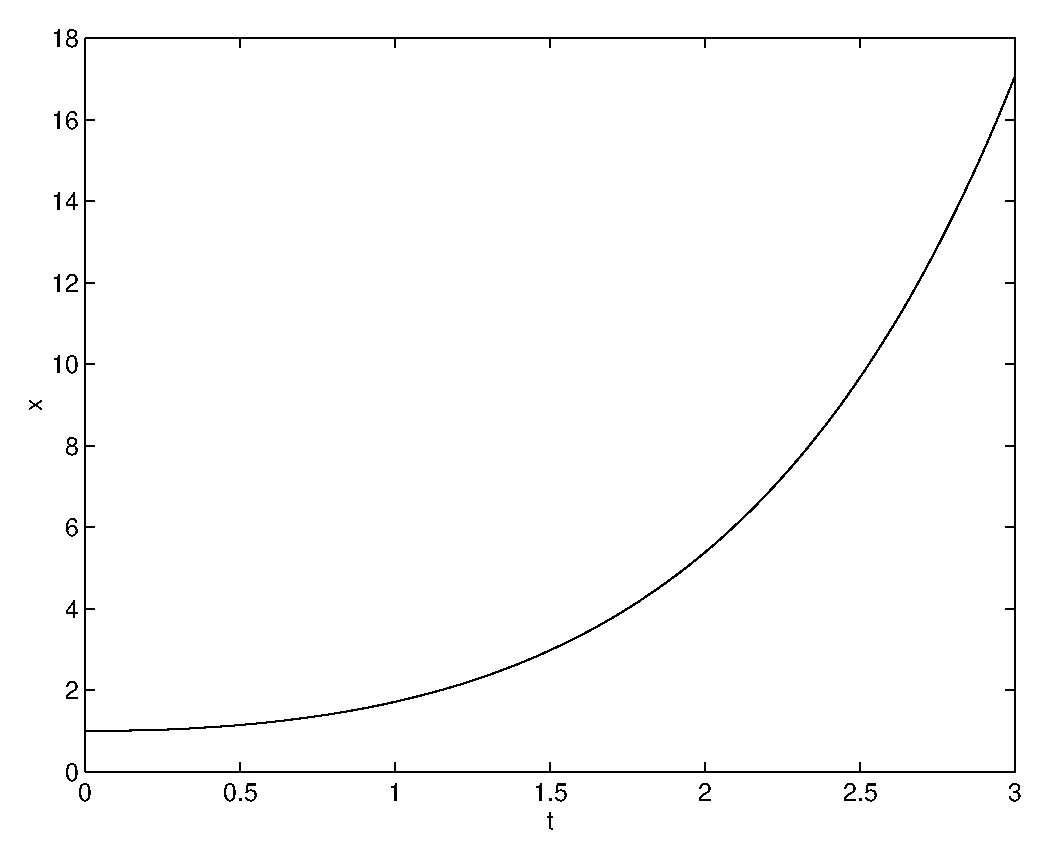
\psfig{file=exfigure/3-1-a78b.eps,width=2.75in}
                       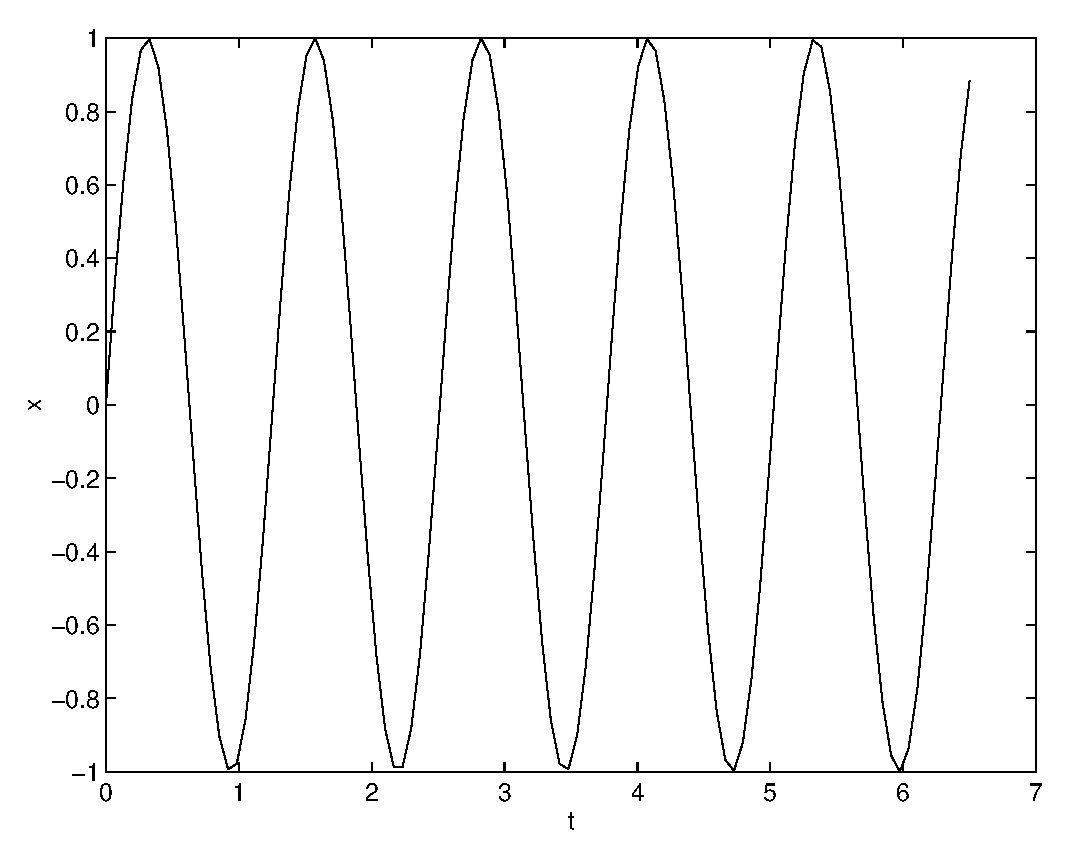
\psfig{file=exfigure/3-1-a78d.eps,width=2.75in}}
	\centerline{Figure~\ref{c3.1.a78b}\hspace{2.1in} Figure~\ref{c3.1.a78d}}
\end{figure}

\exer{c3.1.9}
\ans After two years, an account at Statewide returns more interest than
the Intrastate account.  However, after only one year, the Intrastate
account returns more.

\soln To find the return from each account, use the formula for
compound interest:
\[
P(t) = P_0\left(1 + \frac{r}{N}\right)^{Nt}
\]
If you deposit your money at Statewide, $P_0 = \$4\mbox{,}990$ because of the
fine.  Interest is compounded four times a year, so $N = 4$.  The interest
rate is 8\%, so $r = 0.08$.
After two years, an account at Statewide returns
\[
P_{S}(2) = \$4\mbox{,}990\left(1 + \frac{0.08}{4}\right)^{2(4)} = 
\$5\mbox{,}846.58
\]
If you deposit your money at Intrastate, $r = 0.0775$.  Interest is
compounded daily, so $N = 365$.  So, after two years, the account returns
\[
P_{I}(2) = \$5\mbox{,}000\left(1 + \frac{0.0775}{365}\right)^{2(365)} = 
\$5\mbox{,}838.19.
\]
After only 1 year, however,
\[
P_{S}(1) = \$4\mbox{,}900\left(1 + \frac{0.08}{4}\right)^{4} = \$5\mbox{,}401.37
\]
at Statewide, and
\[
P_{I}(1) = \$5\mbox{,}000\left(1 + \frac{0.0775}{365}\right)^{365} = 
\$5\mbox{,}402.87
\]
at Intrastate.



\subsection*{Section~\protect{\ref{S:3.2}} Graphing Solutions to Differential
Equations}
\rhead{S:3.2}{GRAPHING SOLUTIONS TO DIFFERENTIAL EQUATIONS}

\exer{c3.2.1A} \ans The solution is increasing at the initial point.

\soln At $x(1)=2$, $\dot{x}=x-t=2-1=1>0$.  Therefore, $x(t)$ is increasing
near $t=1$.

\exer{c3.2.1C} \ans The solution is increasing at the initial point.

\soln At $x(1)=2$, $\dot{x}=x^2-tx=4-2=2>0$.  Therefore, $x(t)$ is increasing
near $t=1$.

\exer{c3.2.2A} The sketch should resemble Figure~\ref{c3.2.2A}.

\exer{c3.2.2C} The sketch should resemble Figure~\ref{c3.2.2C}.

\begin{figure}[th]
     \centerline{%
     \psfig{file=exfigure/4-2-5.eps,width=2.75in}
     \psfig{file=exfigure/4-2-7.eps,width=2.75in}}
        \centerline{Figure~\ref{c3.2.2A}\hspace{2.1in} Figure~\ref{c3.2.2C}}
\end{figure} 

\exer{c3.2.3A} Nonautonomous.

\exer{c3.2.3C} Autonomous.

\exer{c3.2.a01a}
To graph the system, enter {\tt dfield5} and change the equation to
{\tt x$'$ = x*t}, and set the range of $x$ to $[-1,1]$ and the range
of $t$ to $[0,2]$.  Then, use keyboard input or mouse to graph
several trajectories.  Sample trajectories are shown in
Figure~\ref{c3.2.a01a}.

\begin{figure}[htb]
                       \centerline{%
                       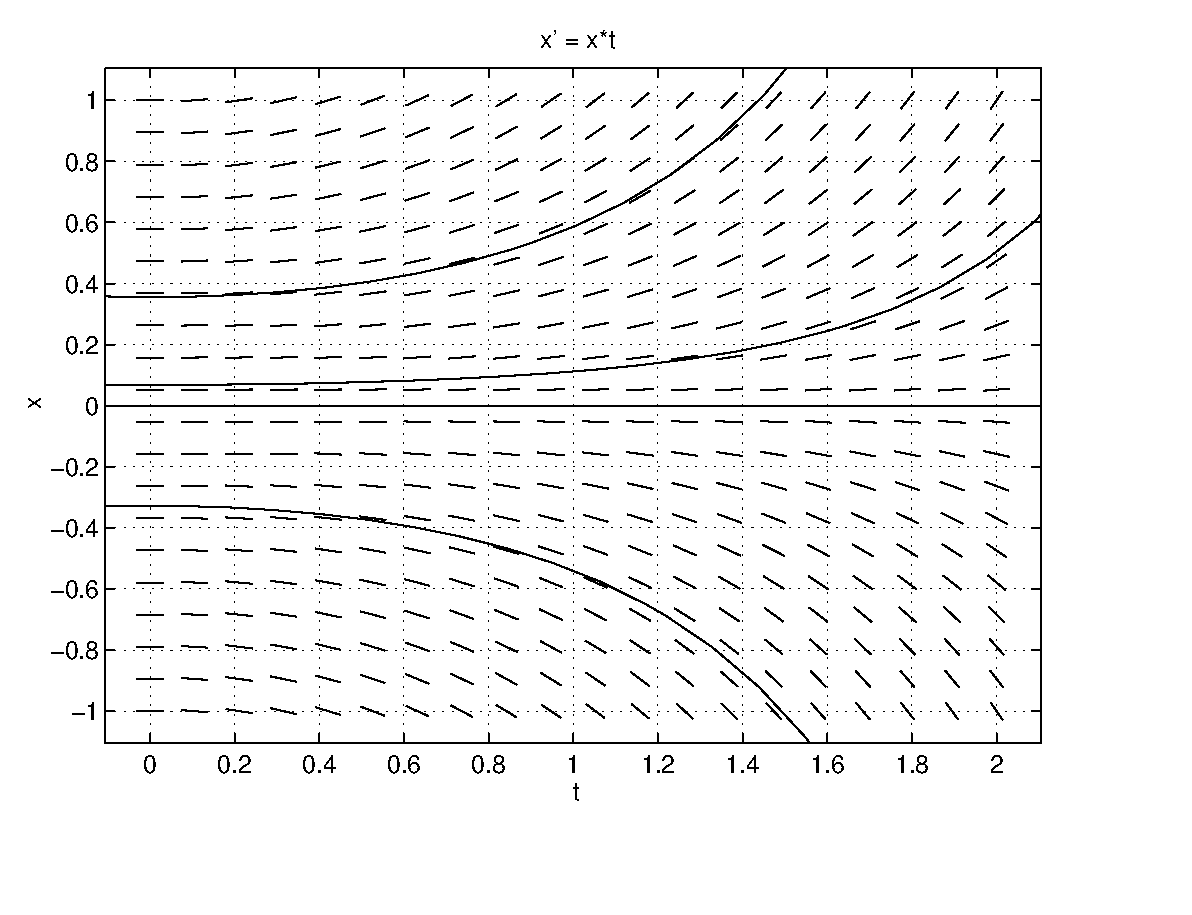
\psfig{file=exfigure/3-2-a01a.eps,width=3.0in}}
                \exercap{c3.2.a01a}
\end{figure}

\exer{c3.2.a01c}
To graph the system, enter {\tt dfield5} and change the equation to
{\tt x$'$ = x - sin(t)}, and set the range of $x$ to $[-4.4]$ and the
range of $t$ to $[-2,10]$.  Sample trajectories are shown in
Figure~\ref{c3.2.a01c}.

\begin{figure}[htb]
                       \centerline{%
                       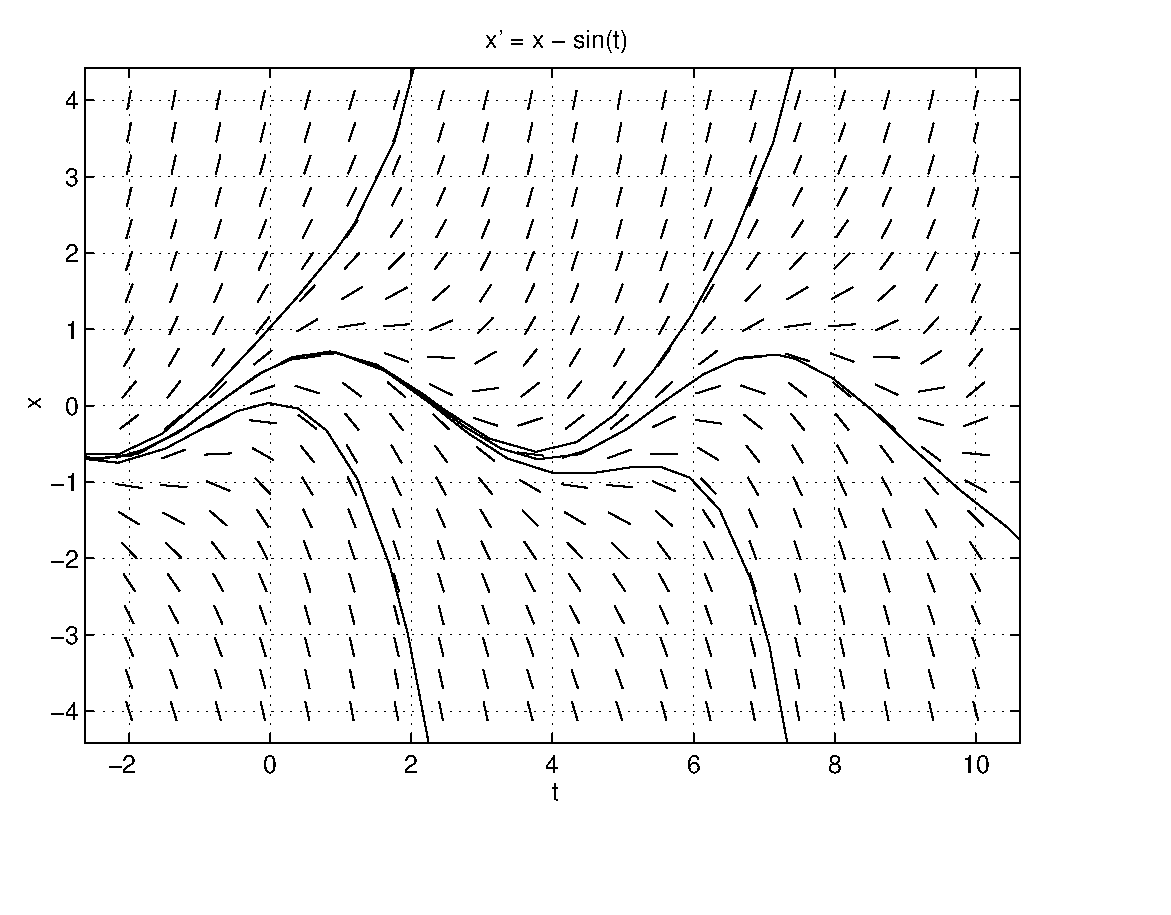
\psfig{file=exfigure/3-2-a01c.eps,width=3.0in}}
                \exercap{c3.2.a01c}
\end{figure}

\exer{c3.2.2}
Figure \ref{c3.2.2}a graphs $\frac{dx}{dt} = x^2 -tx +2t$ with the
initial value $x(-1) = -1$.  Zooming in on the graph shows that the
minimum value of $x$ on the interval $-2 \leq t \leq 1$ is $x \approx
-1.39$.  The Figure \ref{c3.2.2}b shows eight trajectories of
$\frac{dx}{dt} = x^2 -tx +2t$.

\begin{figure}[htb]
                       \centerline{%
                       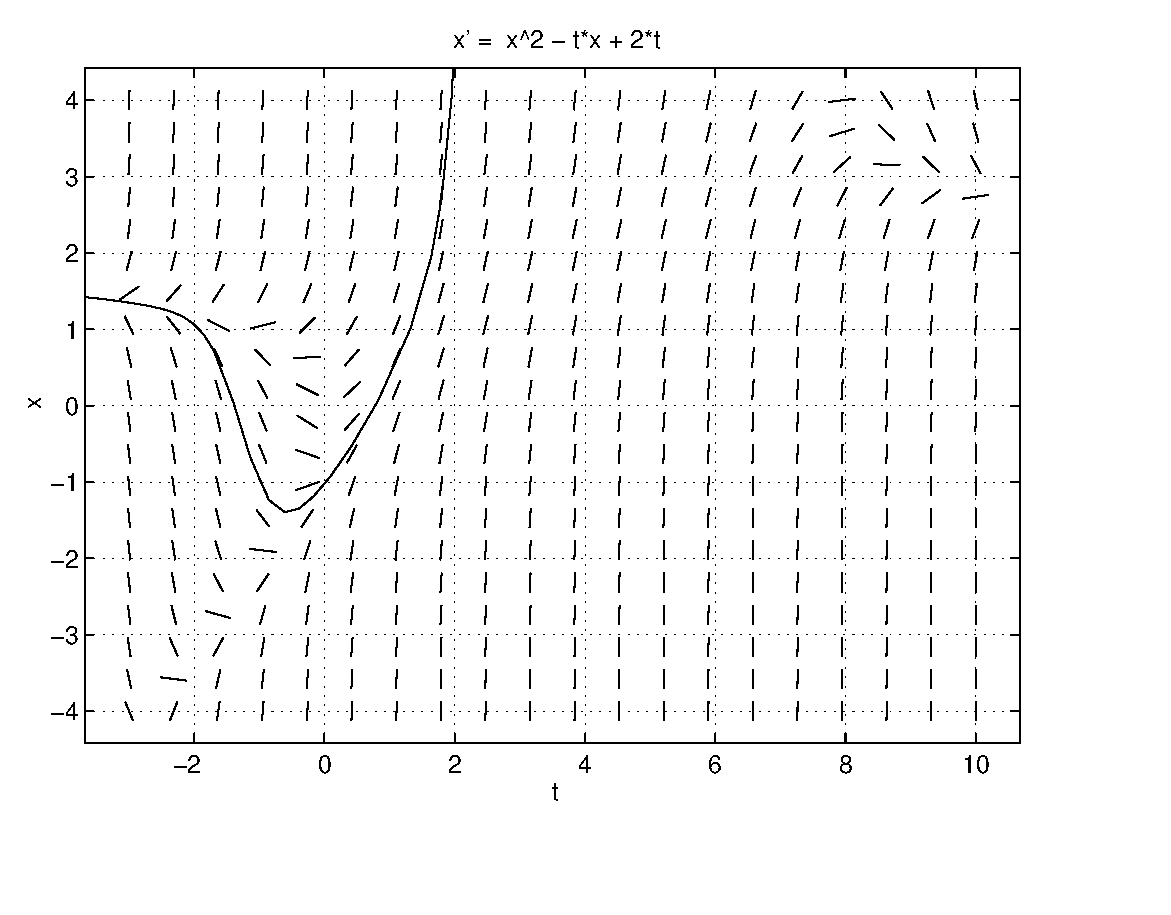
\psfig{file=exfigure/3-2-2a.eps,width=2.75in}
                       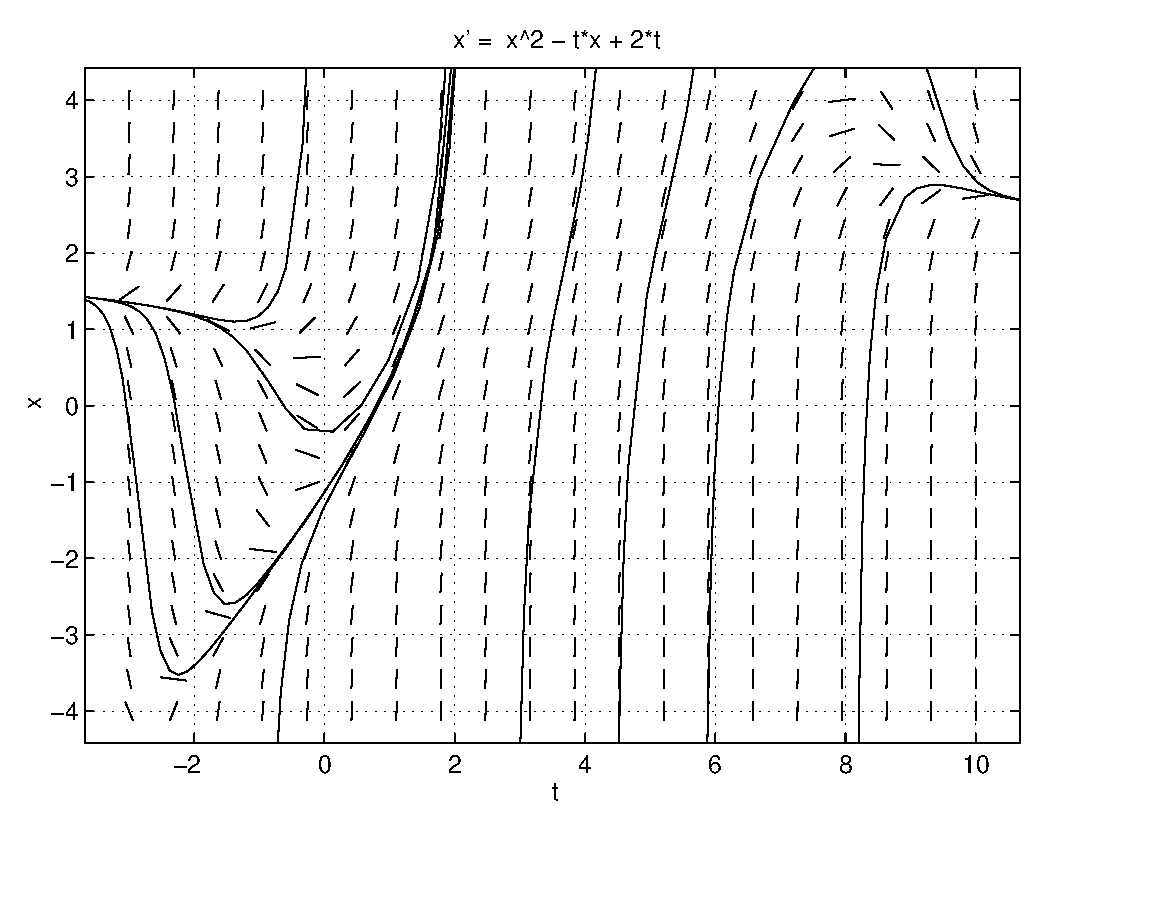
\psfig{file=exfigure/3-2-2b.eps,width=2.75in}}
		\exercaptwo{c3.2.2}
\end{figure}

\exer{exer:at}
(a) The {\tt dfield5} estimate is $x(137) = 273.989$, found by zooming
in on the graph shown in Figure~\ref{exer:at}.  This figure shows the
direction field for $\frac{dx}{dt} = \frac{x}{x - t}$ with the desired
initial condition $x(2) = 3$ on the interval $0 \leq t \leq 150$, $0
\leq x \leq 300$.

(b) In order to verify that the equation $x(t) = t + \sqrt{t^2 - 3}$
is a solution to
\[
\begin{array}{rcl}
\frac{dx}{dt} & = & \frac{x}{x - t} \\
x(2) & = & 3\end{array}
\]
we must show that both of these conditions are valid for the equation.
To show that the first condition holds, take the derivative of $x(t)$.
\[
\frac{dx}{dt} = 1 + \frac{t}{\sqrt{t^2 - 3}} = \frac{t + {\sqrt{t^2 - 
3}}}{\left({\sqrt{t^2 - 3}} + t\right) - t} = \frac{x}{x - t}.
\]
To show that the second condition holds, substitute into the formula for
$x(t)$ to obtain:
\[ x(2) = 2 + \sqrt{2^2 - 3} = 3. \]

(c) The {\tt dfield5} solution coincides with the algebraic solution to at
least 3 decimal places.

\begin{figure}[htb]
                       \centerline{%
                       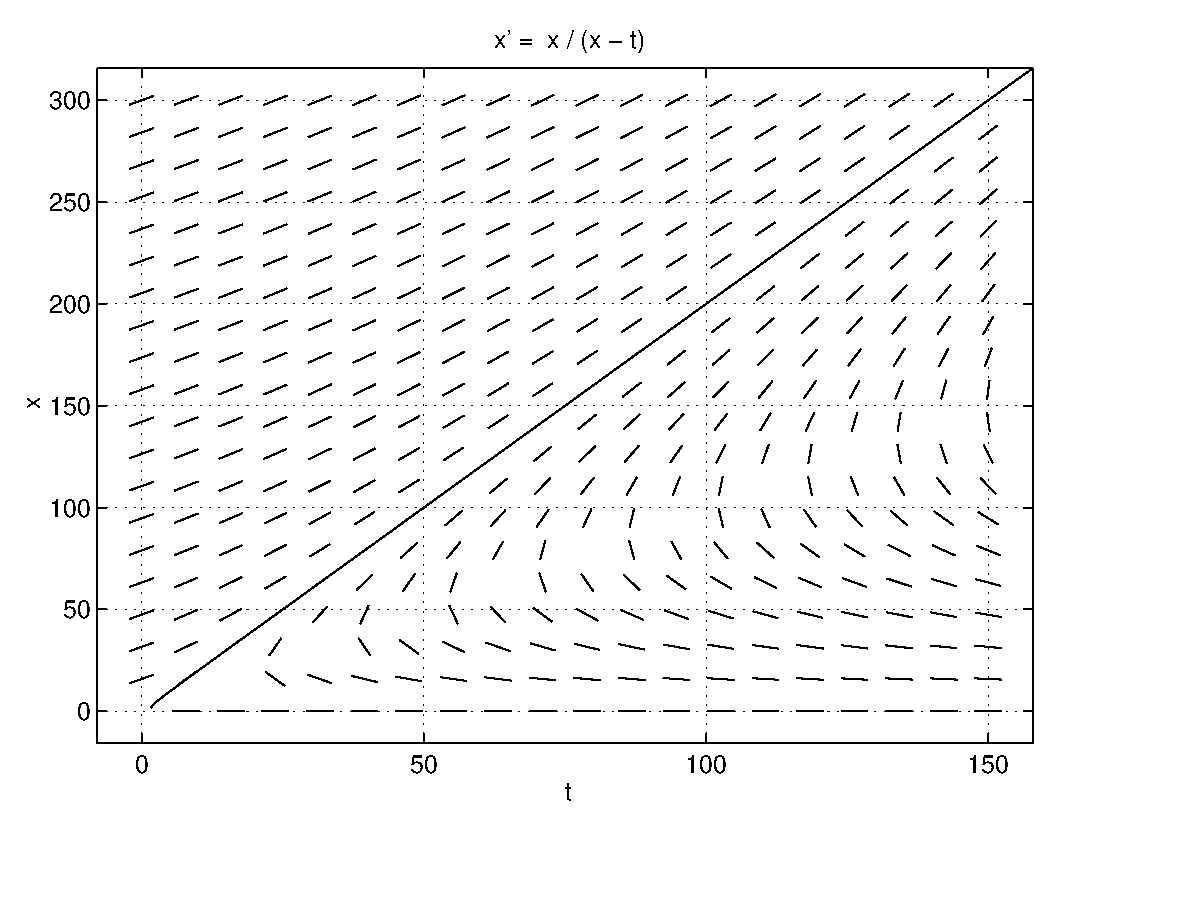
\psfig{file=exfigure/3-2-4.eps,width=3.0in}}
		\exercap{exer:at}
\end{figure}



\subsection*{Section~\protect{\ref{S:PSP&E}} Phase Space Pictures and Equilibria}
\rhead{S:PSP&E}{PHASE SPACE PICTURES AND EQUILIBRIA}

\exer{c3.3.1}
\ans An approximate range of possible initial conditions is
$0.055 \leq x(0) \leq 0.109$. 

\soln Use {\tt pline} to find an appropriate initial condition.
In {\tt pline}, set the value of $\lambda$ to $-0.2$.  Then, set the
integration time to $20$, since integration time corresponds to the
final value of $t$ when the initial value is $0$.  Use either
keyboard input or the mouse to select initial points until you
find one which has an endpoint in the given range. 

\exer{c3.3.3}
\ans The point $x = 1$ is a stable equilibrium when $\lambda > 0$; it is
an unstable equilibrium when $\lambda < 0$. 

\soln We verify this by choosing several values of $\lambda$ in
{\tt pline} and observing that when $\lambda$ is positive, initial values
near $1$ converge to $1$, whereas when $\lambda$ is negative, they do not.

\exer{c3.3.5}
\ans When $\epsilon = -1$, all initial values move towards $x = 0$; whereas
when $\epsilon = 1$, all initial values move away from the origin. 

\soln If we let $g(x) = \epsilon x^3$, we can verify our result using
Theorem~\ref{T:stability1}, which states
that an equilibrium is asymptotically stable if $g'(x) < 0$.  In this case,
\[
g'(x) = 3\epsilon x^2
\]
The expression $3x^2$ is positive for all nonzero real numbers $x$, so
when $x \neq 0$
\[ \begin{array}{ccc}
g'(x) > 0 & \mbox{when} & \epsilon > 0 \\
g'(x) < 0 & \mbox{when} & \epsilon < 0 \end{array}
\]
Therefore, the origin is a stable equilibrium when $\epsilon = -1$ and
an unstable equilibrium when $\epsilon = 1$.

\exer{c3.3.6B}
\ans The points $x=4$ and $x = -2$ are unstable equilibria and the point 
$x = 0$ is a stable equilibrium.

\soln Note that the equilibria for the differential equation
$x' = x^3 - 2x^2 - 8x$ occur at any points where
$g(x) = x^3 - 2x^2 - 8x = x(x - 4)(x + 2) = 0$.
So, the equilibria occur at $x=0$, $x = 4$ and $x = -2$.  Take the
derivative of $g(x)$ at these points, obtaining
\[
\begin{array}{rcccl}
g'(x) & = & 3x^2-4x-8 \\
g'(4) & = & 24 & > & 0 \\
g'(0) & = & -8 & < & 0\\
g'(-2) & = & 12 & > & 0.\end{array}
\]

\exer{c3.3.6D}
\ans The point $x = -3+2\sqrt{2}$ is an unstable equilibrium and 
$x = -3-2\sqrt{2}$ is a stable equilibrium.

\soln Note that the equilibria for the differential equation
$x' = x^2 + 6x + 1$ occur at any points where
$g(x) = x^2 + 6x + 1 = 0$.  So, the equilibria occur at $x =
-3-2\sqrt{2}\approx -5.8284$ and $x = -3+2\sqrt{2}\approx -0.1716$.  Take the
derivative of $g(x)$ at these points, obtaining
\[
\begin{array}{rcccl}
g'(x) & = & 2x + 6 \\
g'(-5.8284) & = & -5.6569 & < & 0 \\
g'(-0.1716) & = & 5.6568 & > & 0.\end{array}
\]

\exer{c3.3.9}
Define a function $y$ such that $y(t) = x(-t)$.  Then, if $x$ is defined by
$\dot{x} = -0.2x$, $y$ can be defined by $\dot{y} = 0.2y$.  In closed form,
$x(t) = Ke^{-0.2t}$ and $y(t) = Ke^{0.2t}$ for some constant $K$.  Let $t_0
= 20$, that is, let $x(20) = x_0 = y(20)$.  Then, by definition,
$x(0) = x(20 - 20) = x(t_0 - 20) = y(t_0 + 20) = y(40)$.  So, to find the
lower bound of the range of possible values of $x_0$, set $x_0 = 0.001$.
Then, $0.001 = y(20) = Ke^4$, so $K \approx 0.0000183$, and $x(0) = Ke^8
\approx 0.0546$.  This agrees with the solution found in
Exercise~\ref{c3.3.1}.

\exer{c3.3.10a} \ans Autonomous.

\soln  The differential equation is autonomous because the line field 
directions are identical all values of $t$.  Equilibria occur at $x$ values 
where the line field is horizontal.  The phase line can be drawn from the 
direction information.  See Figure~\ref{c3.3.10a}.

\begin{figure}[ht]
     \centerline{%
     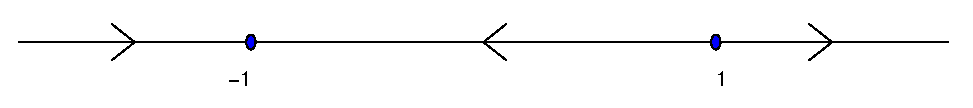
\psfig{file=exfigure/phasea.eps,width=2.0in}}
      \exercap{c3.3.10a}
\end{figure} 

\exer{c3.3.10c} Nonautonomous.



\subsection*{Section~\protect{\ref{sec:sov}} Separation of Variables}
\rhead{sec:sov}{SEPARATION OF VARIABLES}

\exer{c14.1.1a} \ans Separation of variables can be used on this differential
equation; the functions are $g(x) = x^{1/2}$ and $h(t) = \cos t$.

\exer{c14.1.1c} \ans Separation of variables cannot be used on this
differential equation.

\exer{c14.1.5a} \ans The solution to the given initial value problem is
\[
x(t) = -e^{-3t}.
\]
\soln Use separation of variables., as follows.  rewrite the differential 
equation as
\[
\frac{1}{x}\frac{dx}{dt} = -3.
\]
Integrate both sides, obtaining 
\[
\ln|x| = -3t + C.
\]
Determine $C$ using the initial condition $(t_0,x_0)=(0,-1)$, obtaining
$C=0$.  Exponentiate to obtain 
\[
|x(t)| = e^{-3t}
\]
and use the initial condition to determine the correct sign.

\exer{c14.1.5c} \ans The solution to the given initial value problem is
\[
x(t) = \frac{1}{9}(2t^{3/2} + 1)^2.
\]
\soln Rewrite the differential equation as 
\[
\frac{1}{2\sqrt{x}}\frac{dx}{dt} = \sqrt{t}.
\]
Integrate both sides to obtain
\[
\sqrt{x} = \frac{2}{3}t^{3/2} + C.
\]
Determine $C$ using the initial condition $(t_0,x_0)=(1,1)$, that is,
\[
C = \sqrt{1} - \frac{2}{3}1^{3/2} = \frac{1}{3}.
\]
Therefore
\[
\sqrt{x} = \frac{1}{3}(2t^{3/2} + 1).
\]
Solve for $x$ to obtain the closed form solution to the initial value problem.

\exer{c14.1.8b} \ans The general solution to the differential equation is 
\[
x(t) = Ke^{5t} - \frac{2}{5}
\]
for some $K \geq 0$.  Note that $x(t) = x_0 = -\frac{2}{5}$ is a constant
solution.

\soln The differential equation can be written $\frac{dx}{dt} = g(x)h(t)$,
where $g(x) = 5x + 2$ and $h(t) = 1$.  Then $x(t)$ satisfies
\[
G(x(t)) = H(t) + C.
\]
For $x(t) \neq -\frac{2}{5}$,
\[
G(x) = \int\frac{1}{g(x)}dx = \int\frac{1}{5x + 2}dx = \frac{1}{5}\ln|5x + 2|
\AND
H(x) = \int dt = t.
\]
So, $x(t)$ satisfies
\[
\frac{1}{5}\ln|5x + 2| = t + C.
\]
Solve for $x(t)$ to obtain the solution to the differential equation.

\exer{c14.1.11a} Figure~\ref{c14.1.11a}a shows several trajectories of the
differential equation.  All solutions limit on $x = 0$ in backward
time.  Trajectories with positive initial values of $x$ increase in
forward time, while trajectories with negative initial values of $x$
decrease in forward time.  Figure~\ref{c14.1.11a}b shows several trajectories
of the linear differential equation $\dot{x} = x$.  The trajectories of this
system also limit on $x = 0$ in backward time and diverge in forward time.

\begin{figure}[htb]
                       \centerline{%
                       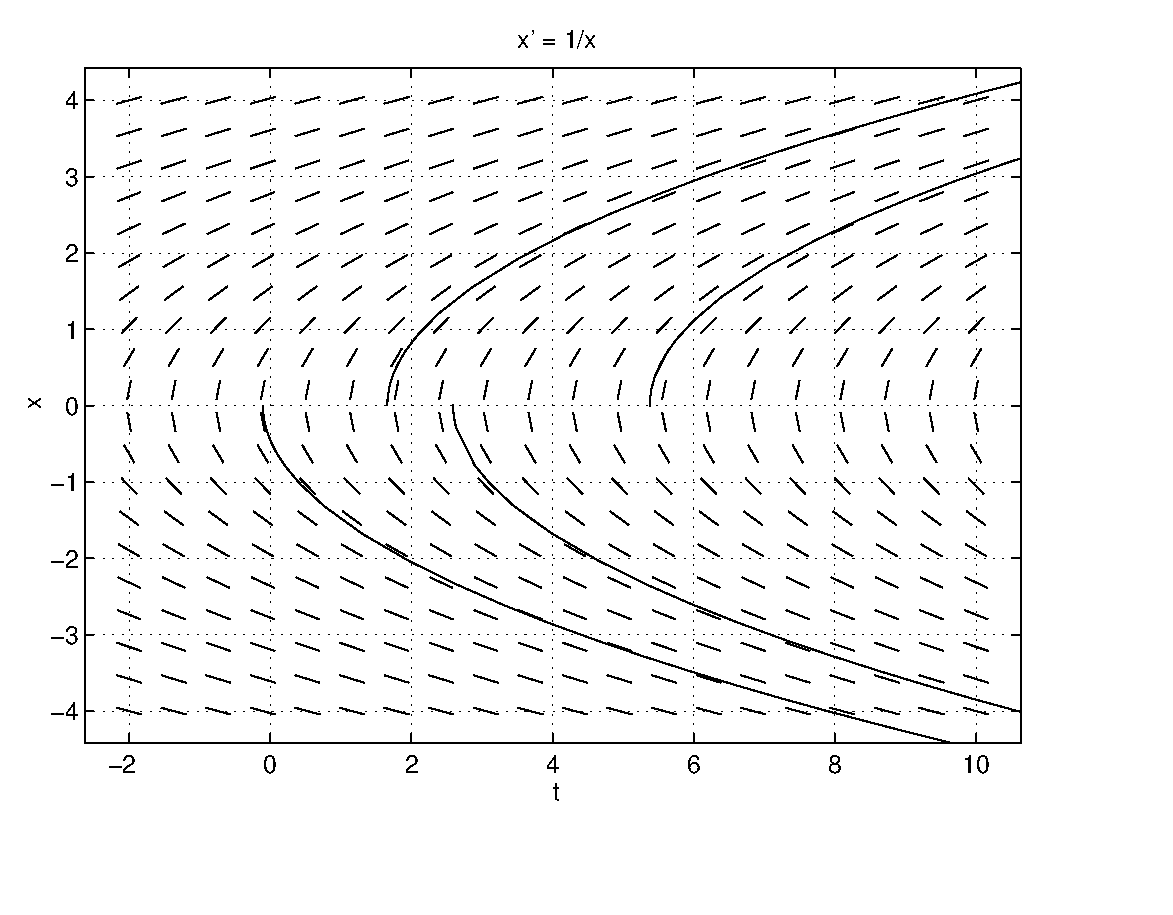
\psfig{file=exfigure/14-1-11aa.eps,width=2.75in}
                       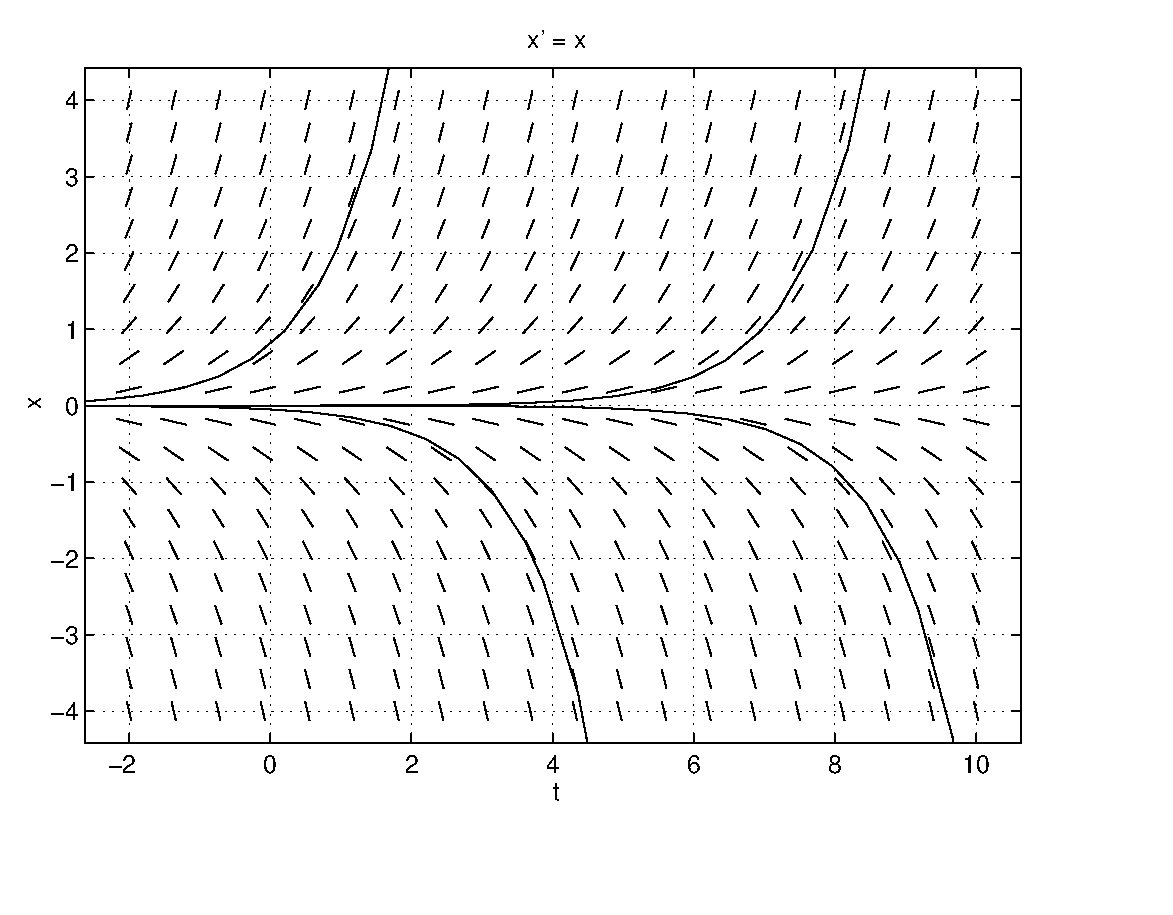
\psfig{file=exfigure/14-1-11ab.eps,width=2.75in}}
                \exercaptwo{c14.1.11a}
\end{figure}

\exer{c14.1.11c} Figure~\ref{c14.1.11c} shows several trajectories of the
differential equation.  The equation has a constant solution at $x(t)
= x_0 = 0$.

\begin{figure}[htb]
                       \centerline{%
                       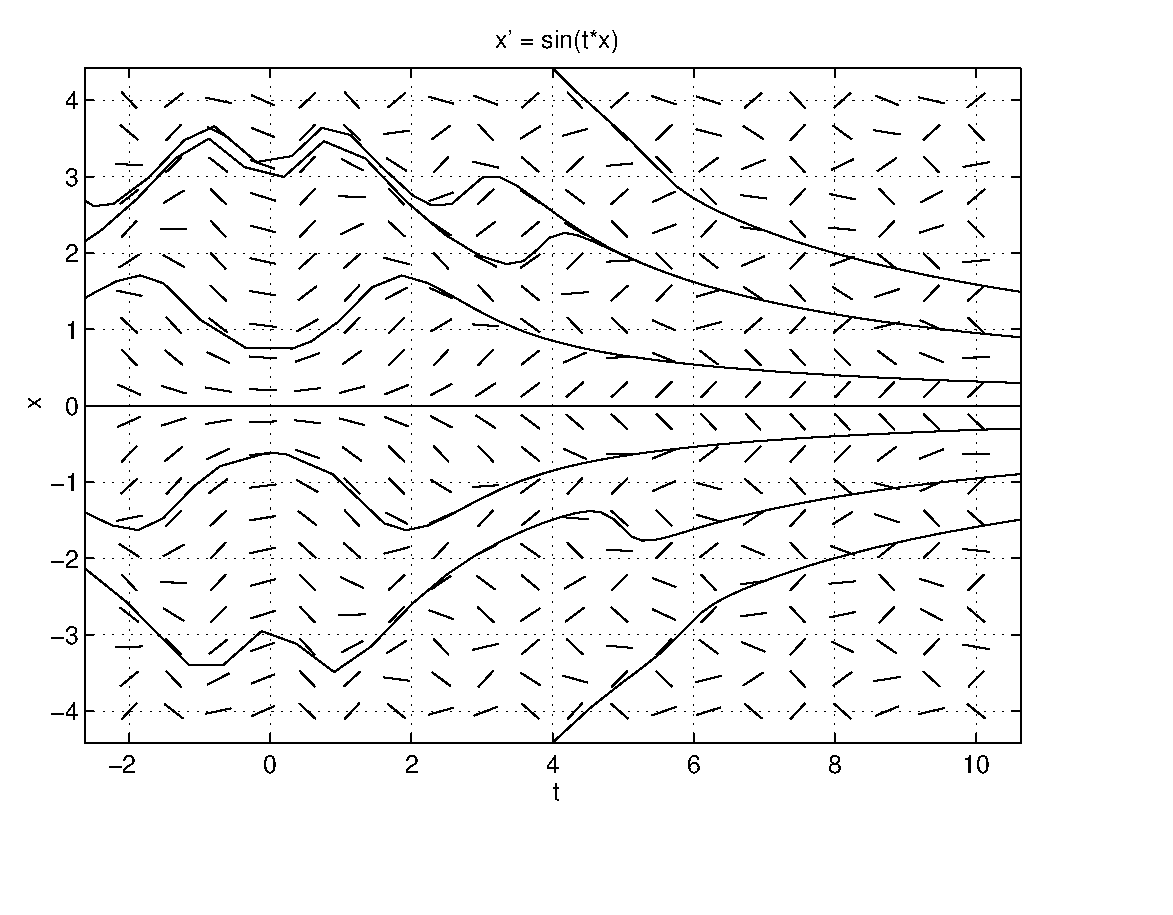
\psfig{file=exfigure/14-1-11c.eps,width=3.0in}}
                \exercap{c14.1.11c}
\end{figure}

\exer{c14.1.11e} Figure~\ref{c14.1.11e} shows several trajectories of the
differential equation.  The equation has constant solutions $x(t) = 0$,
$x(t) = -1$ and $x(t) = 1$.  All solutions with initial conditions
$x_0 = x(t_0)$ such that $|x_0| < 1$ limit on $x = 0$ in backward time and
limit on $x = 1$ or $x = -1$ in forward time.  All other solutions limit
on $x = 1$ or $x = -1$ in backward time and diverge in forward time.

\begin{figure}[htb]
                       \centerline{%
                       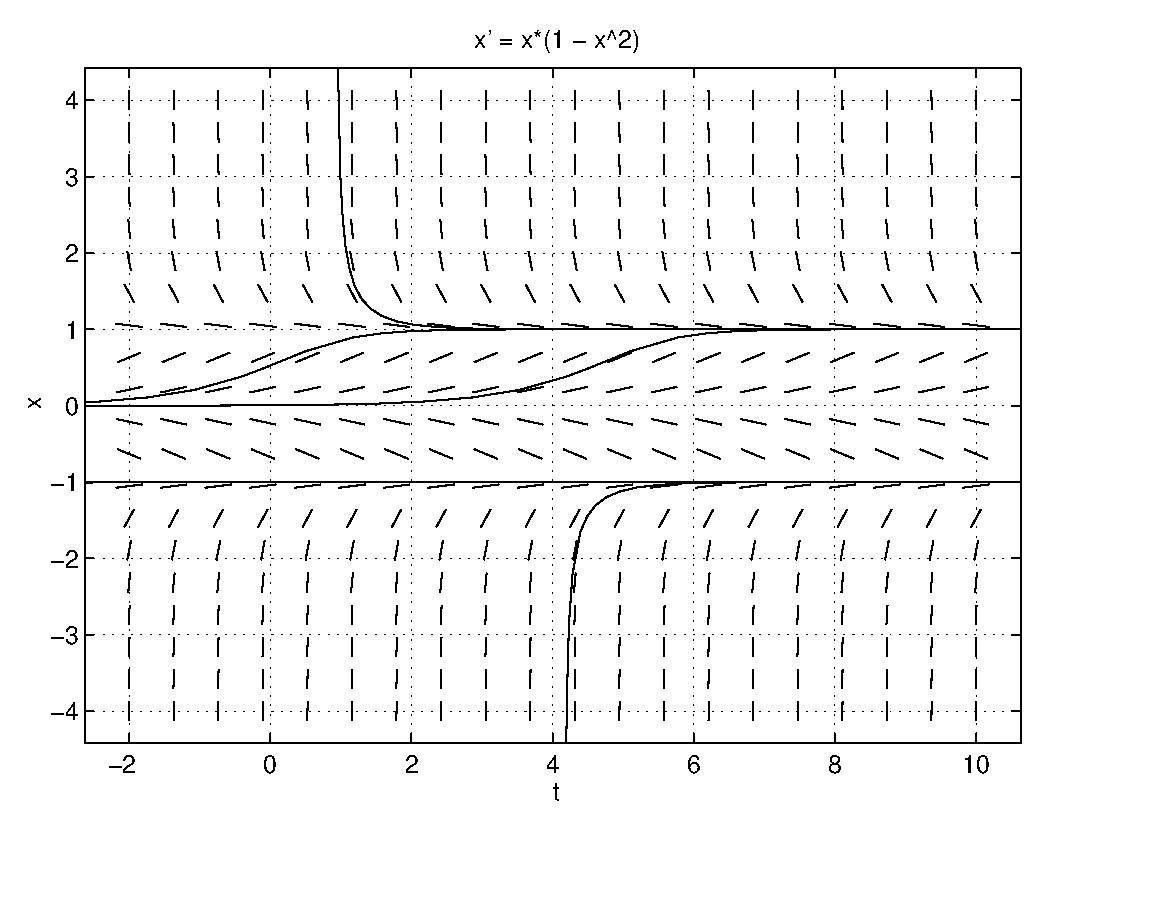
\psfig{file=exfigure/14-1-11e.eps,width=3.0in}}
                \exercap{c14.1.11e}
\end{figure}

\exer{c14.1.17} Figure~\ref{c14.1.17}a shows the graph of the initial
value problem with $0.8 \leq t \leq 1.2$.  Figure~\ref{c14.1.17}b shows
the same initial value problem with $0.5 \leq t \leq 1.2$.  In
backward time, $x(t)$ limits on the origin at $t \approx 0.7$, at
which point the trajectory ends.

\begin{figure}[htb]
                       \centerline{%
                       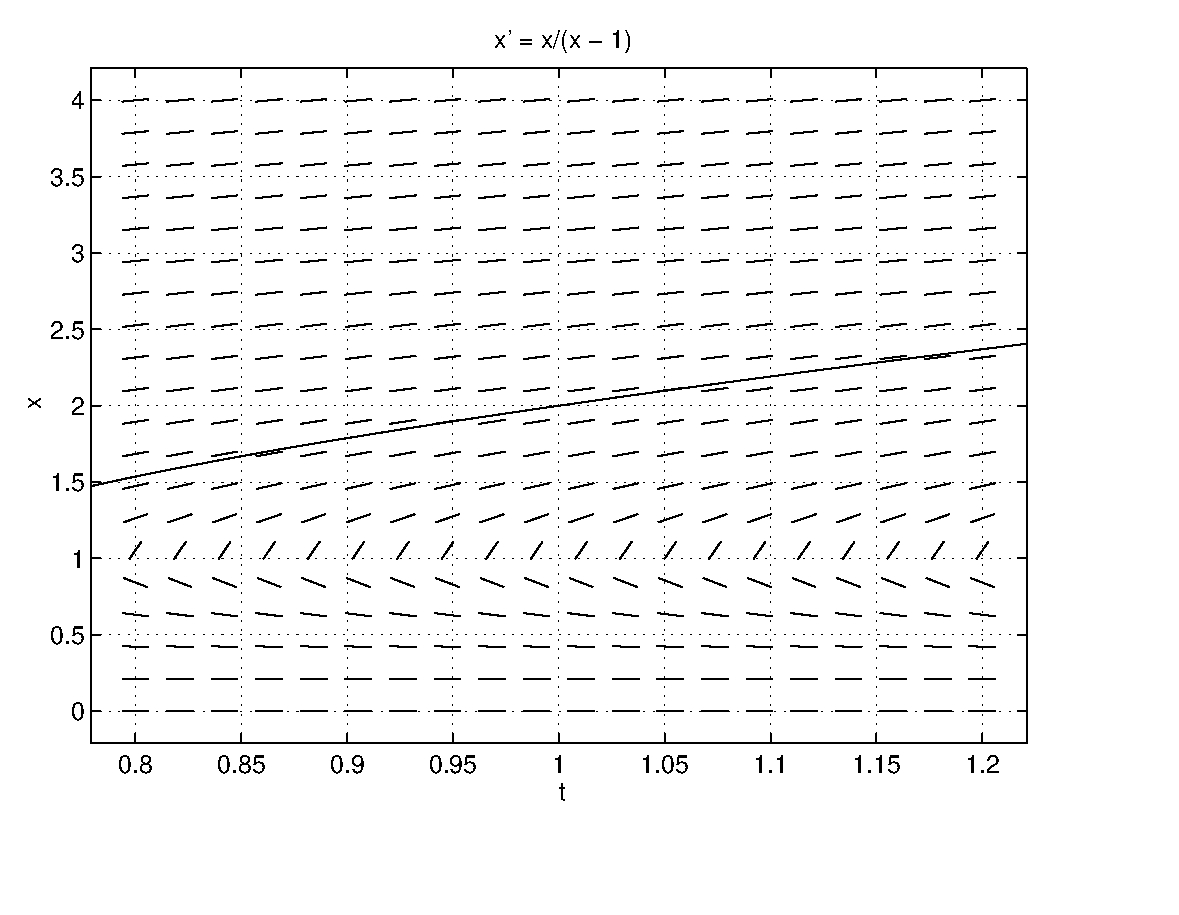
\psfig{file=exfigure/14-1-17a.eps,width=2.75in}
                       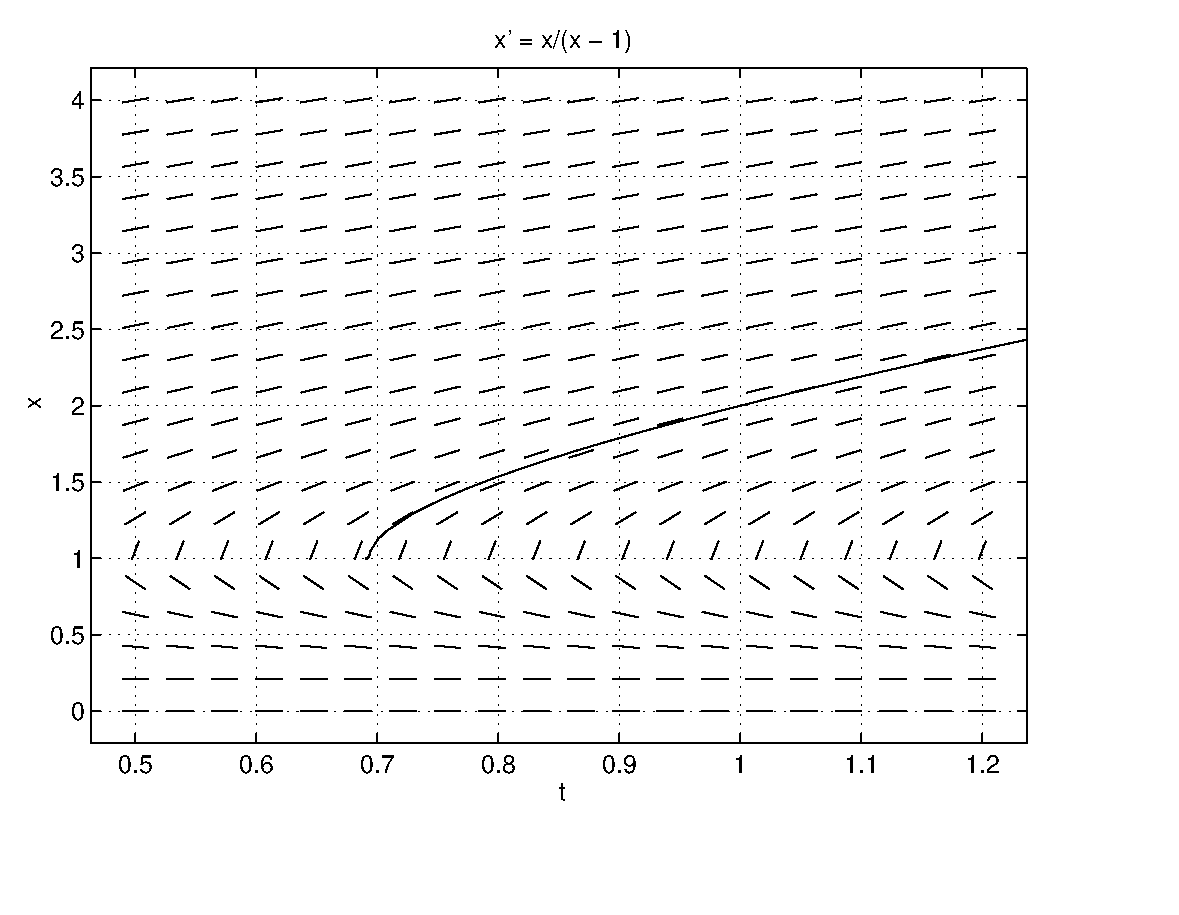
\psfig{file=exfigure/14-1-17b.eps,width=2.75in}}
                \exercaptwo{c14.1.17}
\end{figure}



\newpage
\subsection*{Section~\protect{\ref{sec:UncoupledLS}} Uncoupled Linear
Systems of Two Equations}
\rhead{sec:UncoupledLS}{UNCOUPLED LINEAR SYSTEMS OF TWO EQUATIONS}

\exer{c3.5.1A} \ans There are two equilibria at $(0,0)$ and $(1,1)$.

\soln Find the equilibria by solving the equations
\begin{eqnarray*}
\dot{x} & = & x-y\\
\dot{y} & = & x^2-y.
\end{eqnarray*}
Substituting $x=y$ from the $1^{st}$ equation into the $2^{nd}$ equation
yields $y^2-y = y(y-1)=0$.  Therefore, $y=0$ or $y=1$.

\exer{E:uncoupleda}
\ans The origin is a saddle.

\soln This uncoupled system is of the form
\[
\begin{array}{rcl}
\frac{dx}{dt}(t) & = & Ax(t) \\
\frac{dy}{dt}(t) & = & Dy(t)\end{array}
\]
If $AD < 0$, then the origin is a saddle.  If $A < 0$ and
$D < 0$, then the origin is a sink.  If $A > 0$ and $D > 0$, then
the origin is a source.  In this case, $AD = -1 < 0$.

\exer{E:uncoupledc} For this system, $A = 0$, so the origin is neither a
saddle, a source nor a sink.  Note that $\frac{dx}{dt} = 0$, so every
point on the $x$-axis is an equilibrium.

\exer{c3.4.3}
We are given $x(0) = \frac{1}{2}$.  Figure \ref{pp_dsp1}
shows that $x$ increases as $t$
increases, and that $x$ limits on $0$ as $t$ decreases.  From
this information, we can sketch a graph of $x(t)$ for the system.
The graph should be similar to Figure \ref{c3.4.3}, which can
be viewed in \Matlab by entering the system in {\tt pplane5},
then choosing ``{\tt x vs.\ t}'' from the graph menu.

\begin{figure}[htb]
                       \centerline{%
                       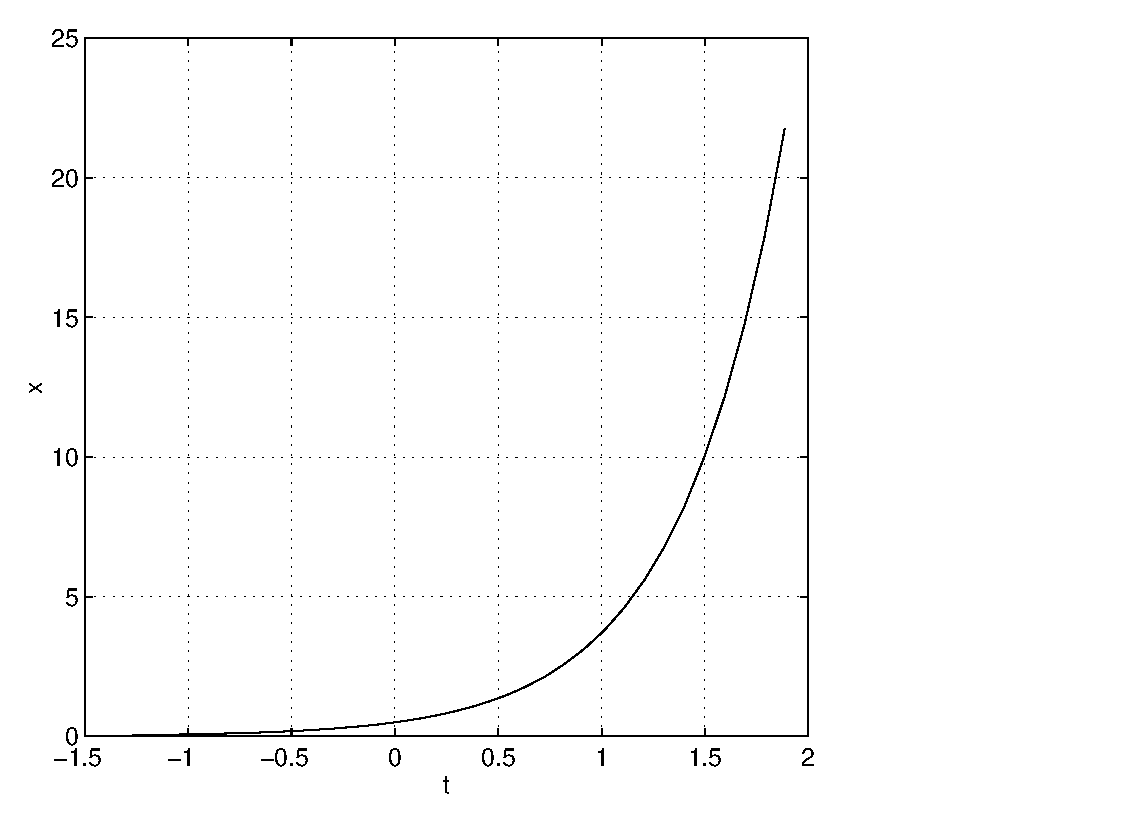
\psfig{file=exfigure/3-4-3.eps,width=3.0in}}
		\exercap{c3.4.3}
\end{figure}

\exer{c3.4.5}
\ans Trajectories approach the origin tangent to the $y$-axis if
$A < D < 0$. 

\soln We can prove this fact by showing that, as $t \rightarrow \infty$,
the tangent direction of the trajectory limits on the $y$-axis.  The
tangent vector of the trajectory $(x(t),y(t))$ at any point is:
\[ \left(\frac{dx}{dt}(t), \frac{dy}{dt}(t)\right) = \left(Ax(t),
Dy(t)\right) = \left(Ax_0e^{At}, Dy_0e^{Dt}\right) =
e^{Dt}\left(Ax_0e^{(A - D)t}, Dy_0\right) \]
The value of $e^{Dt}$ is relevant only to the length of the
tangent and does not affect the direction.  As $t$ approaches
infinity, $e^{(A - D)t}$ approaches $0$, since $A - D < 0$.
Therefore, the limiting tangent direction is
\[ \lim_{t \rightarrow \infty} \left(Ax_0e^{(A - D)t}, Dy_0\right)
= (0, Dy_0), \]
which is on the $y$-axis.  So our conjecture is indeed true.

\exer{c3.4.7}
\ans Sets of identical initial conditions have identical trajectories
for the two systems. 

\soln To see this, graph the systems using {\tt pplane5} and
{\tt dfield5}, then use keyboard input to enter several sets of initial
conditions, as shown in Figures~\ref{c3.4.7}a of the {\tt pplane5} system
and \ref{c3.4.7}b of the {\tt dfield5} system.  To see why this is the case,
note that {\tt pplane5} graphs the uncoupled system
\begin{equation} \label{eq:3.4.7}
\frac{dx}{dt} = 2x \AND \frac{dy}{dt} = -3y.
\end{equation}
This is a parameterized system in three variables $(x(t),y(t),t)$.
We can rewrite this system in two variables $(x(y),y)$, by using the
chain rule as follows:
\[ -\frac{2x}{3y} = \frac{\frac{dx}{dt}}{\frac{dy}{dt}} = \frac{dx}{dy}. \]
Substitute $t$ for $y$ in the new system to verify that \Ref{eq:3.4.7}
is a parameterization of
\[ \frac{dx}{dt} = -\frac{2x}{3t}. \]

\begin{figure}[htb]
			\centerline{%
			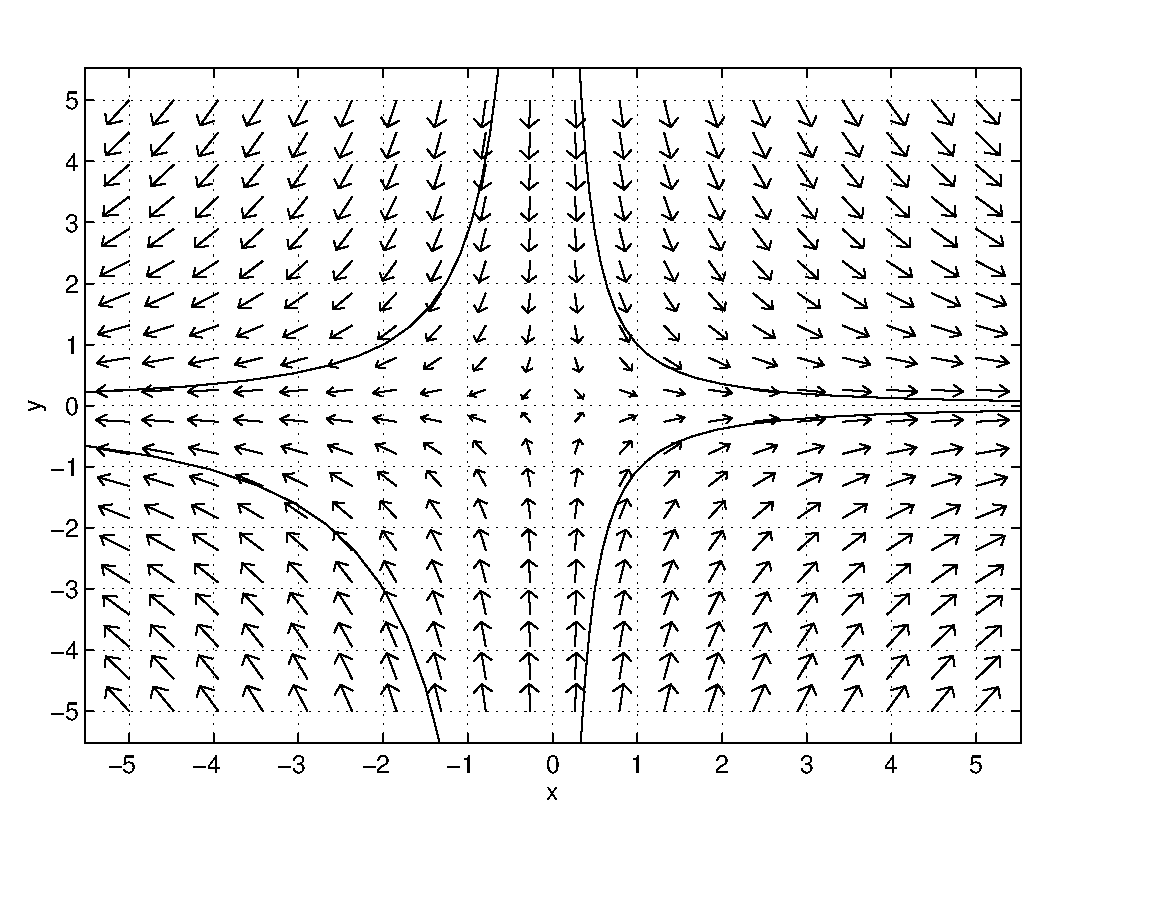
\psfig{file=exfigure/3-4-7a.eps,width=2.75in}
			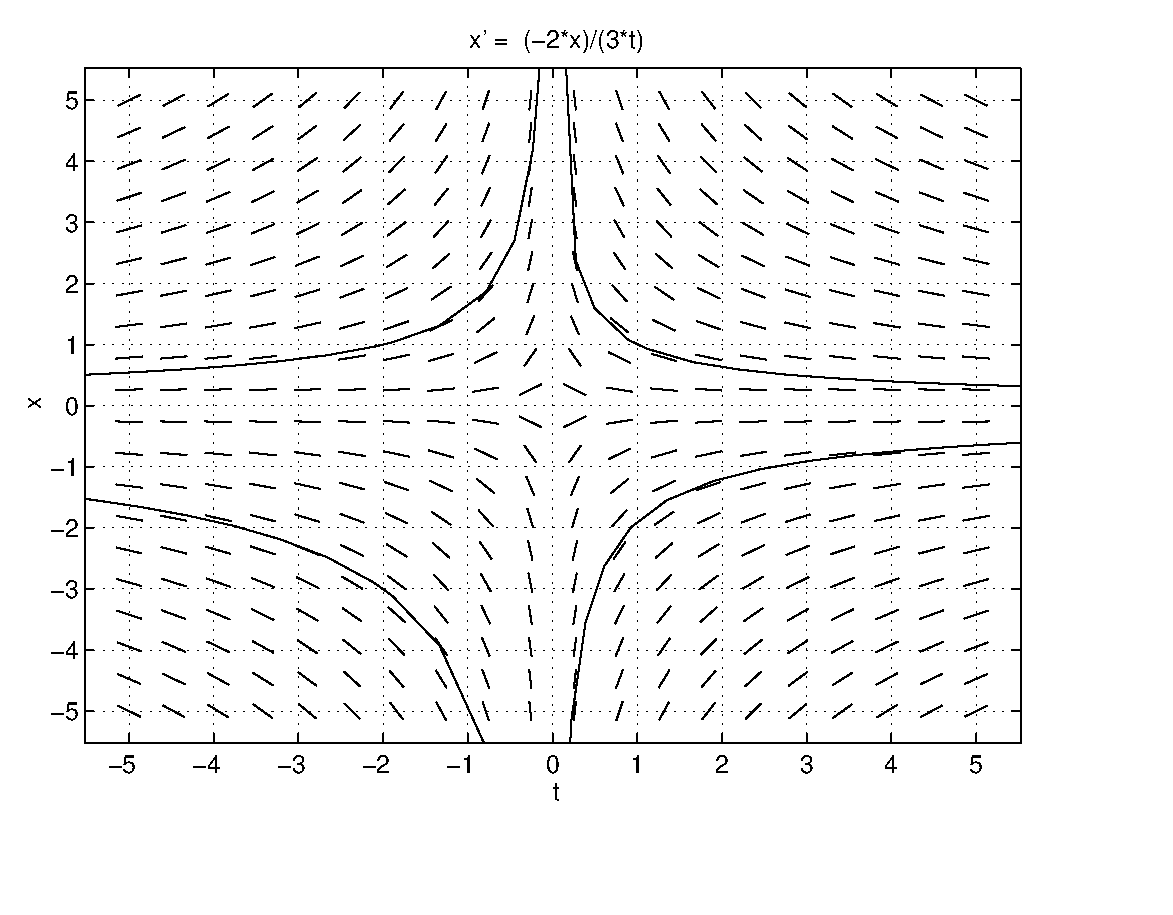
\psfig{file=exfigure/3-4-7b.eps,width=2.75in}}
		\exercaptwo{c3.4.7}
\end{figure}



\subsection*{Section~\protect{\ref{s:3.5}} Coupled Linear Systems}
\rhead{s:3.5}{COUPLED LINEAR SYSTEMS}

\exer{c3.5.a01}
(a) All trajectories converge on the origin when $D < 0$, as shown in
Figure~\ref{c3.5.a01}a, which graphs the system with $D =- 1$;

(b) All trajectories move away from the origin when $D > 0$, as shown in
Figure~\ref{c3.5.a01}b, which graphs the system with $D = 1$

(c) Trajectories form circles around the origin when $D = 0$, as shown in
Figure~\ref{c3.5.a01}c.

\begin{figure}[htb]
                       \centerline{%
                       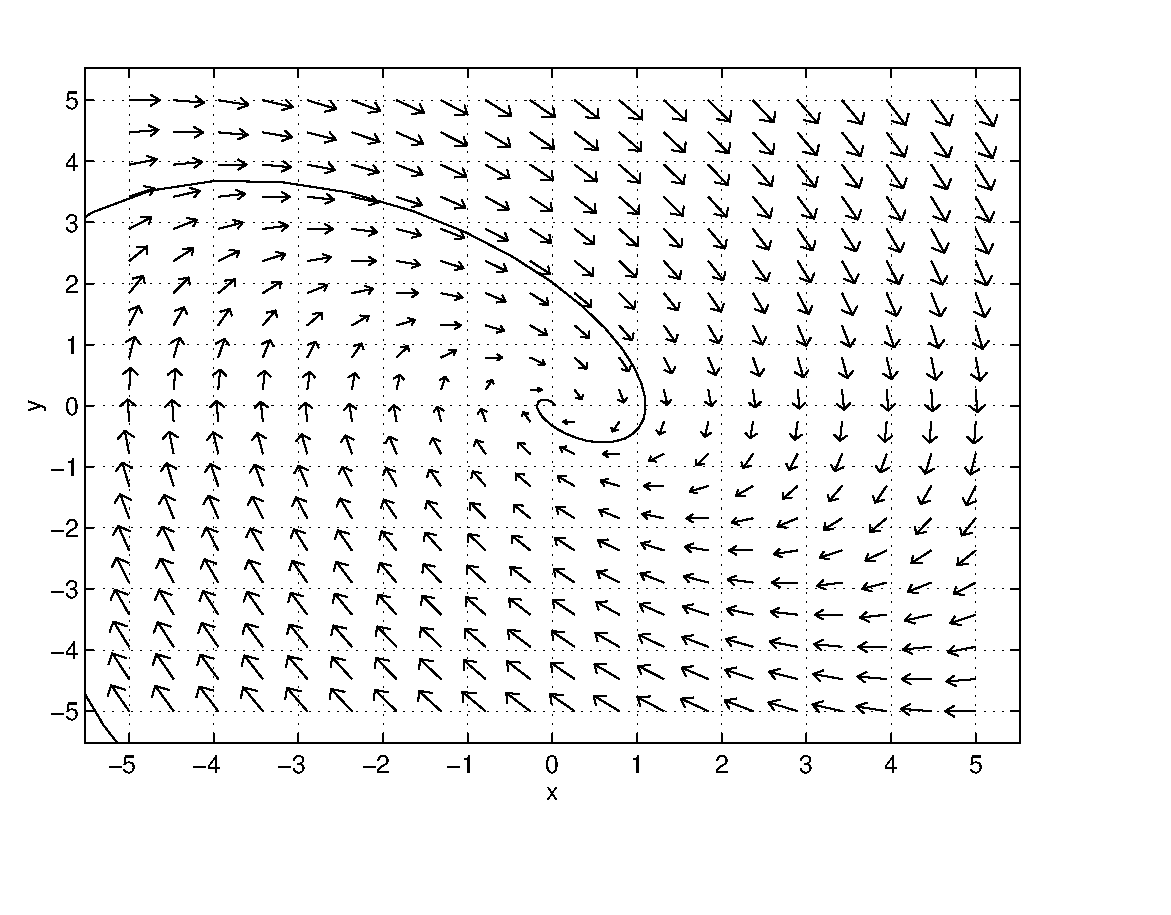
\psfig{file=exfigure/3-5-a01a.eps,width=1.8in}
                       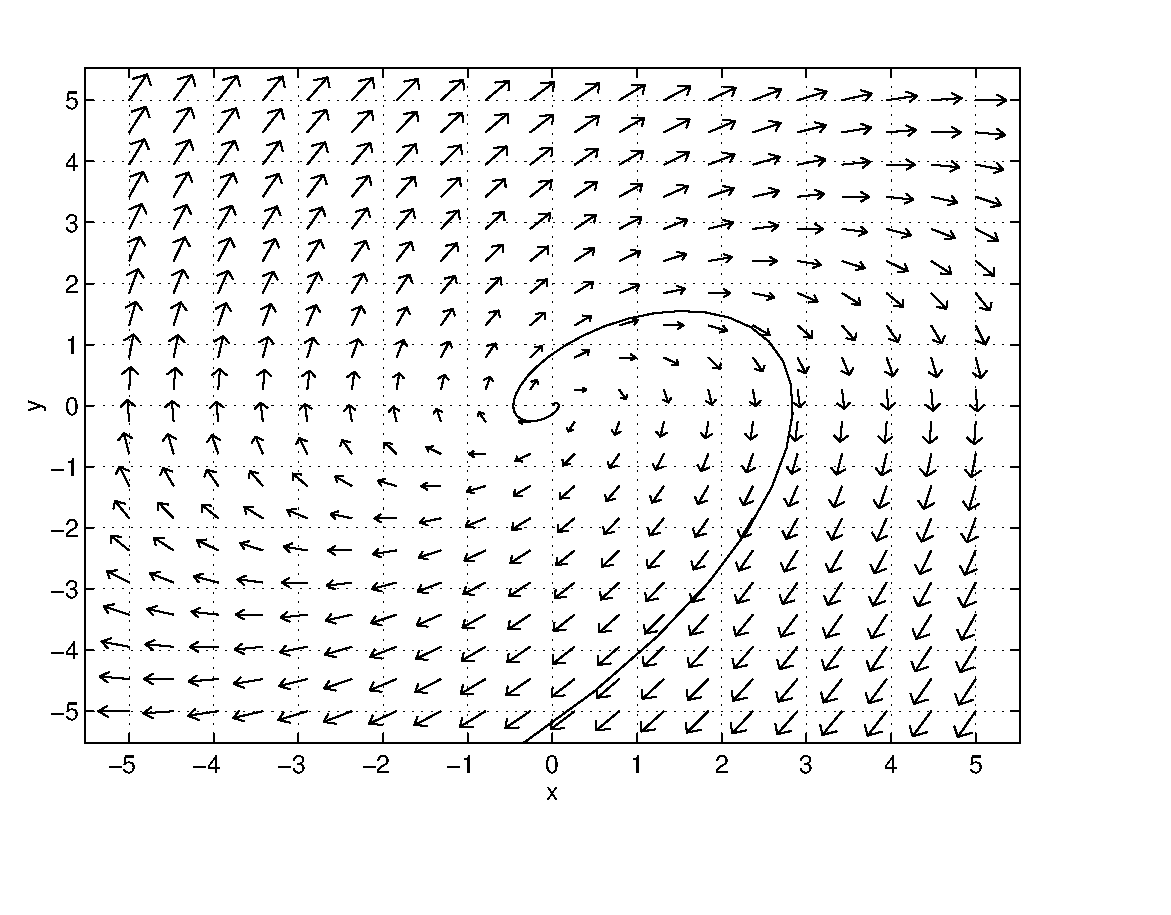
\psfig{file=exfigure/3-5-a01b.eps,width=1.8in}
                       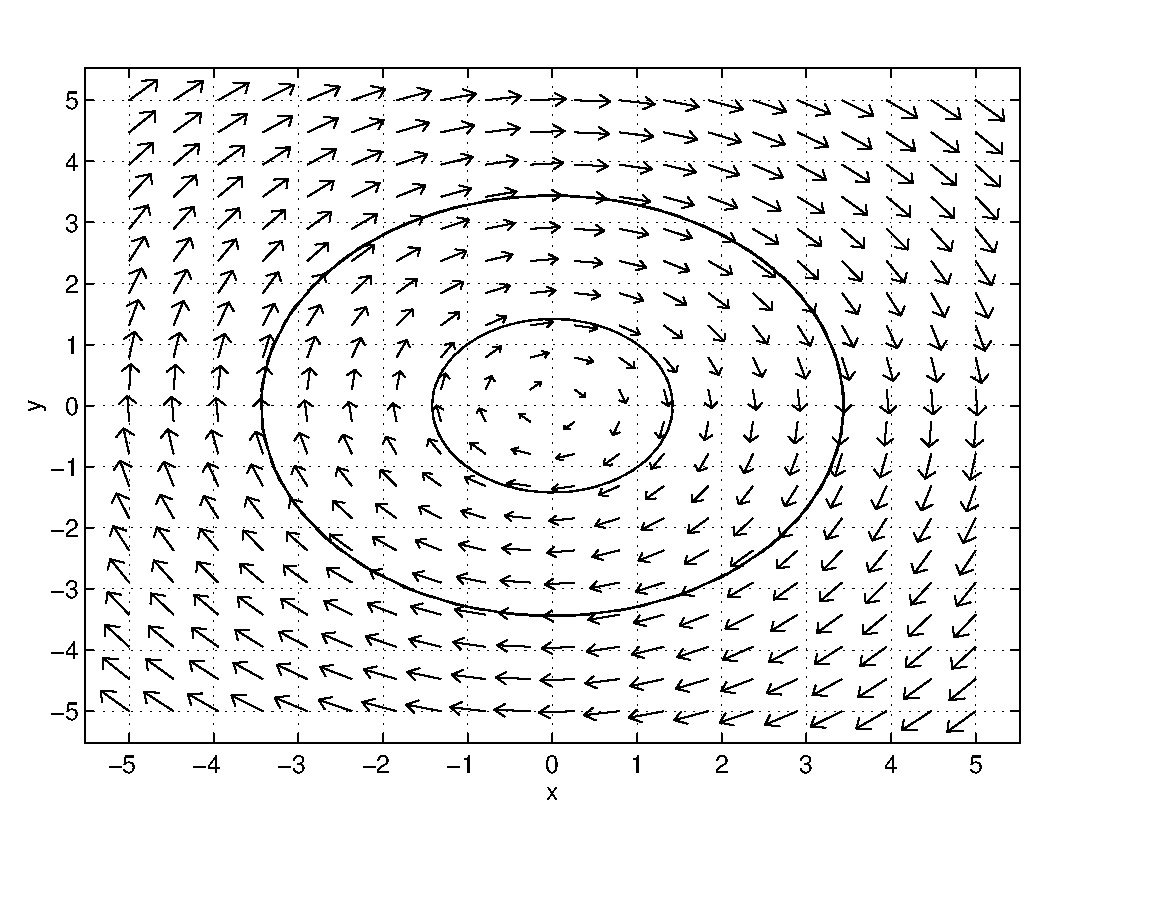
\psfig{file=exfigure/3-5-a01c.eps,width=1.8in}}
	\centerline{$D = -1$\hspace{1.4in}$D = 1$\hspace{1.4in}$D = 0$}
	\exercapthree{c3.5.a01}
\end{figure}

\exer{c3.5.3}
Graphs made in {\tt pplane5} using the {\tt axis('equal')} command
verify these statements regarding linear systems where $A = D$
and $B = C$.  Figure \ref{c3.5.3}a, uses $A = D = -1$ and
$B = C = 2$, and shows four sample trajectories which approach
the line $y = x$ as $t \rightarrow \infty$.  Figure
\ref{c3.5.3}b graphs the linear system with $A = D = -3$
and $B = C = 2$.  It shows four sample trajectories, three of
which approach the origin tangent to $y = x$.  The fourth
trajectory has an initial point $0 < x_0 = -y_0$ and approaches
the origin on the straight line $y = -x$, which is orthogonal
to $y = x$.

\begin{figure}[htb]
                       \centerline{%
                       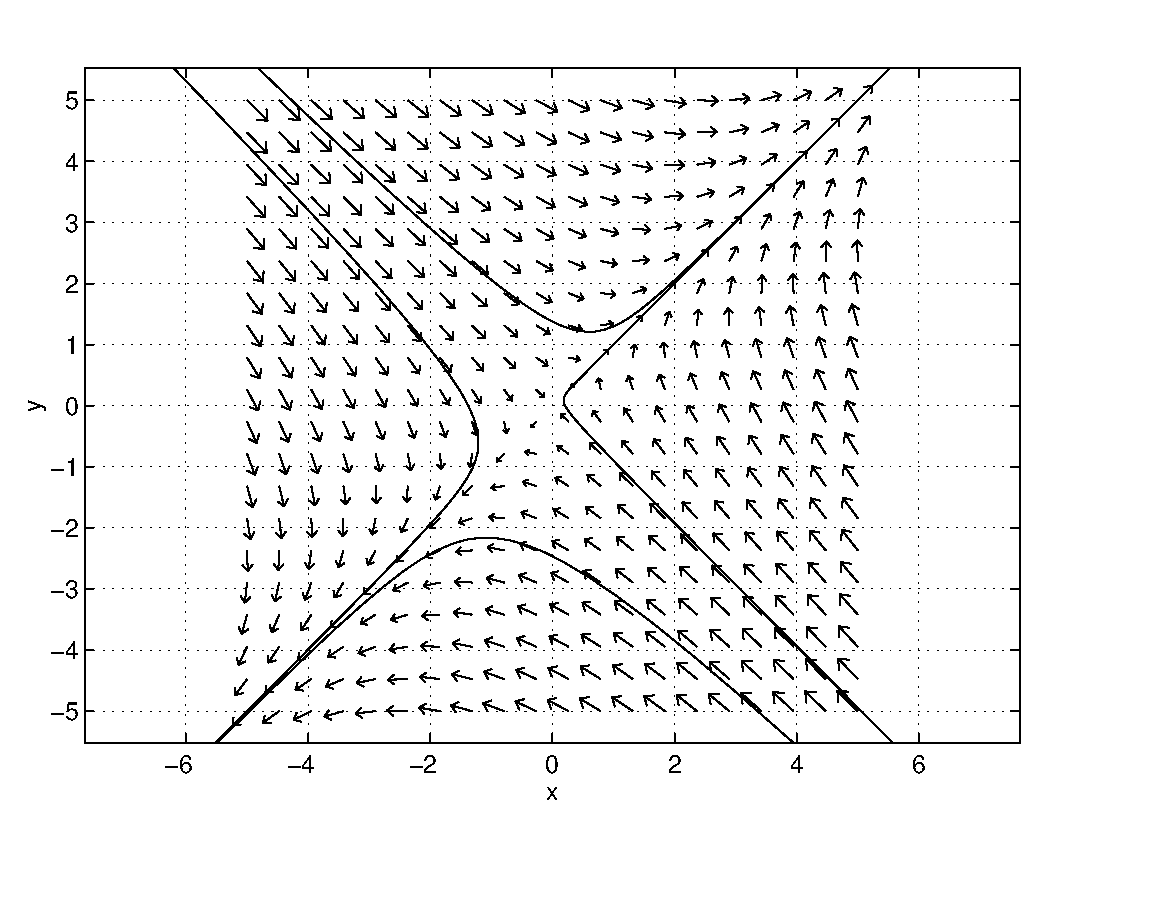
\psfig{file=exfigure/3-5-3a.eps,width=2.75in}
                       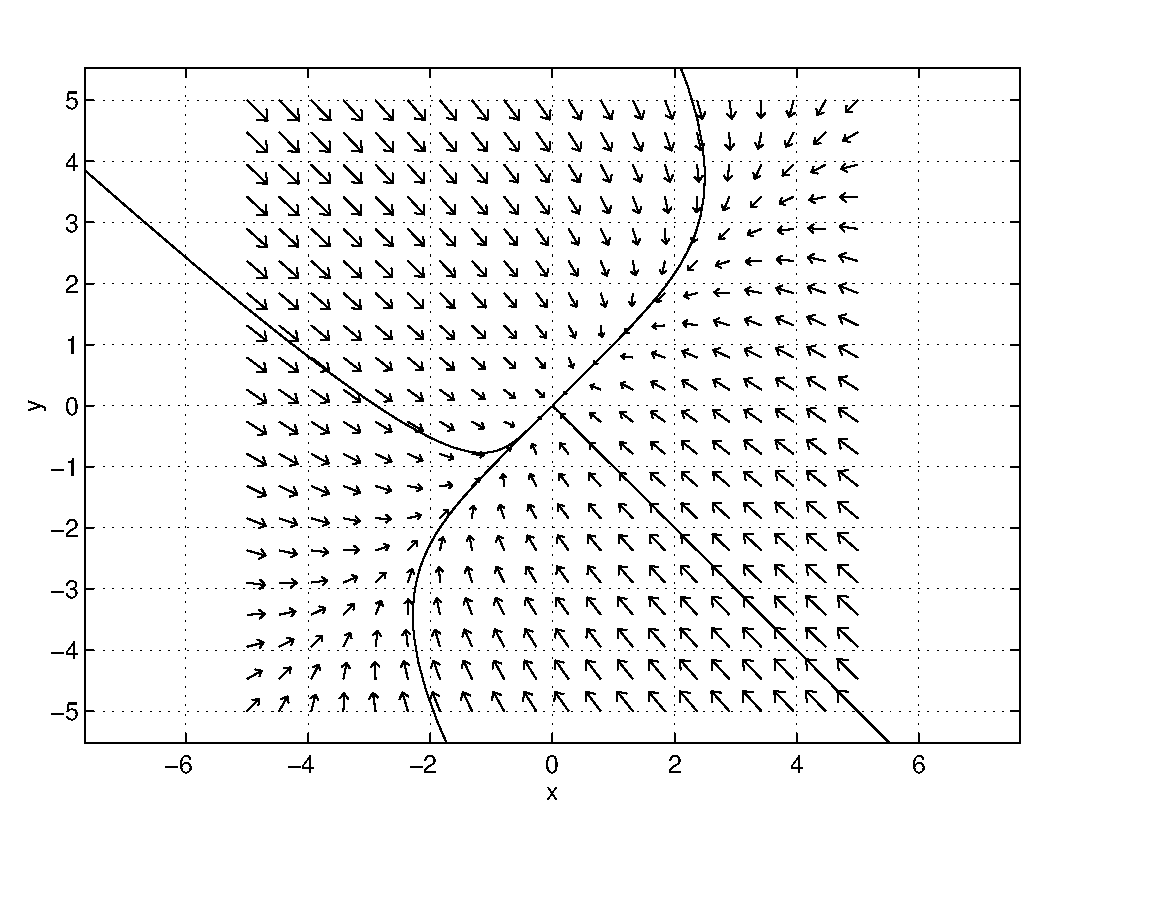
\psfig{file=exfigure/3-5-3b.eps,width=2.75in}}
			\exercaptwo{c3.5.3}	
\end{figure}

\exer{c3.5.5a} \ans Both function pairs are solutions to the given system.

\soln To determine whether $(x_1(t),y_1(t)) = (e^{2t},0)$ is
a solution to the system, compute the left hand sides of the equations:
\[
\frac{dx_1}{dt}(t) = \frac{d}{dt}(e^{2t}) = 2e^{2t} \AND
\frac{dy_1}{dt}(t) = \frac{d}{dt}(0) = 0.
\]
Then compute the right hand sides of the equations:
\[
2x_1(t) + y_1(t) = 2e^{2t} + 0 = 2e^{2t} \AND
3y_1(t) = 3(0) = 0.
\]
Since the left hand side of each equation equals the right hand side, the
equations are consistent, and the pair of functions is a solution.

\para Similarly, to determine whether $(x_2(t),y_2(t)) = (e^{3t},e^{3t})$
is a solution to the system, compute the left hand sides of the equations:
\[
\frac{dx_2}{dt}(t) = \frac{d}{dt}(e^{3t}) = 3e^{3t} \AND
\frac{dy_2}{dt}(t) = \frac{d}{dt}(e^{3t}) = 3e^{3t}.
\]
Then compute the right hand sides of the equations:
\[
2x_2(t) + y_2(t) = 2e^{3t} + e^{3t} = 3e^{2t} \AND
3y_2(t) = 3e^{3t}.
\]
Since the left hand side of each equation equals the right hand side, the
equations are consistent, and the pair of functions is a solution.

\exer{c3.5.5c} \ans The function pair $(e^t\sin{t},e^t\cos{t})$ is a
solution to the system, while the function pair $(3e^t,-2e^t)$ is not.

\soln To determine whether $(x_1(t),y_1(t)) = (3e^t,-2e^t)$ is
a solution to the system, compute the left hand sides of the equations:
\[
\frac{dx_1}{dt}(t) = \frac{d}{dt}(3e^t) = 3e^t \AND
\frac{dy_1}{dt}(t) = \frac{d}{dt}(-2e^t) = -2e^t.
\]
Then compute the right hand sides of the equations:
\[
x_1 + y_1 = 3e^t - 2e^t = e^t \AND
-x_1 + y_1 = -3e^t - 2e^t = -5e^t.
\]
Since $\frac{dx_1}{dt} \neq x_1 + y_1$ and $\frac{dy_1}{dt} \neq -x_1 + y_1$,
the pair of functions is not a solution.

\para Similarly, to determine whether $(x_2(t),y_2(t)) =
(e^t\sin{t},e^t\cos{t})$ is a solution to the system, compute the left
hand sides of the equations:
\[
\frac{dx_2}{dt}(t) = \frac{d}{dt}(e^t\sin{t}) = 
e^t\sin{t} + e^t\cos{t} \AND
\frac{dy_2}{dt}(t) = \frac{d}{dt}(e^t\cos{t}) =
e^t\cos{t} - e^t\sin{t}.
\]
Then compute the right hand sides of the equations:
\[
x_2(t) + y_2(t) = e^t\sin{t} + e^t\cos{t} \AND
-x_2(t) + y_2(t) = -e^t\sin{t} + e^t\cos{t}.
\]
Since the left hand side of each equation equals the right hand side, the
equations are consistent, and the pair of functions is a solution.



\subsection*{Section~\protect{\ref{S:IVP&E}} The Initial Value Problem and
Eigenvectors}
\rhead{S:IVP&E}{THE INITIAL VALUE PROBLEM AND EIGENVECTORS}

\exer{c4.1.5}
\arraystart
\[
\left(\begin{array}{r} \dps\frac{dx_1}{dt}(t) \\ 
\dps\frac{dx_2}{dt}(t)\end{array}\right) =
\left(\begin{array}{rr} 4 & 5 \\ 2 & -3\end{array}\right)
\left(\begin{array}{r} x_1(t) \\ x_2(t)\end{array}\right)
\]
\arrayfinish

\exer{c4.5.1}
(a) In order to determine that $Y(t)$ is a solution
to \Ref{e:Ceqn}, substitute $Y(t)$ into both sides of the 
equation $\frac{dX}{dt} = CX$:
\[
\frac{dY}{dt}
= \frac{d}{dt}\left(e^{2t}\vectwo{1}{0}\right)
= \frac{d}{dt}\cvectwo{e^{2t}}{0}
= \cvectwo{2e^{2t}}{0};
\]
\[
CY(t)
= \mattwo{2}{3}{0}{-1}\cvectwo{e^{2t}}{0}
= \cvectwo{2e^{2t}}{0}.
\]
Similarly, show that $Z(t)$ is a solution:
\[
\frac{dZ}{dt}
= \frac{d}{dt}\left(e^{-t}\vectwo{1}{-1}\right)
= \frac{d}{dt}\cvectwo{e^{-t}}{-e^{-t}}
= \cvectwo{-e^{-t}}{e^{-t}};
\]
\[
CZ(t)
= \mattwo{2}{3}{0}{-1}\cvectwo{e^{-t}}{-e^{-t}}
= \cvectwo{-e^{-t}}{e^{-t}}.
\]

(b) Again, verify that $X(t) = 2Y(t) - 14Z(t)$ is a solution to
\Ref{e:Ceqn} by substituting into both sides of the equation and
noting that the values are equal:
\[
\frac{dX}{dt}
= \frac{d}{dt}\left(2e^{2t}\vectwo{1}{0} - 14e^{-t}\vectwo{1}{-1}\right)
= \frac{d}{dt}\cvectwo{2e^{2t} - 14e^{-t}}{14e^{-t}} 
= \cvectwo{4e^{2t} + 14e^{-t}}{-14e^{-t}};
\]
\[
CX(t) = C\left(2Y(t) - 14Z(t)\right)
= C\left(\cvectwo{2e^{2t}}{0} - \cvectwo{14e^{-t}}{-14e^{-t}}\right)
= \cvectwo{4e^{2t} + 14e^{-t}}{-14e^{-t}}.
\]

(c) As demonstrated in Section~\ref{S:Superposition}, if
$Y(t)$ and $Z(t)$ are both solutions to
\Ref{e:Ceqn}, then $X(t) = \alpha Y(t) + \beta Z(t)$ is also
a solution to \Ref{e:Ceqn}.

(d) \ans 
\[
X(t) = 2e^{2t}\vectwo{1}{0} + e^{-t}\vectwo{1}{-1}.
\]

\soln Note that
\[ X(t) = \alpha Y(t) + \beta Z(t) = \alpha e^{2t}\vectwo{1}{0}
+ \beta e^{-t}\vectwo{1}{-1} \]
is a solution to \Ref{e:Ceqn}.  Substitute the value
$X(0) = (3,-1)^t$  into the equation to find a solution with that
initial condition:
\[
\vectwo{3}{-1} = X(0) = \alpha\vectwo{1}{0} +
\beta\vectwo{1}{-1}.
\]
We now have the linear system:
\[ \begin{array}{rrrrr}
3 & = & \alpha & + & \beta \\
-1 & = & & & -\beta \end{array} \]
which we can solve to find $\alpha = 2$ and $\beta = 1$.

\exer{c4.5.3}
\ans Let
\[ v_1 = \vectwo{1}{1} \AND v_2 = \vectwo{1}{-1}. \]
The vector $v_1$ is an eigenvector of $C$ with corresponding
eigenvalue $a + b$, and $v_2$ is an eigenvector with eigenvalue $a - b$.

\soln Calculate
\[ Cv_1 = \mattwo{a}{b}{b}{a}\vectwo{1}{1} = \vectwo{a + b}{a + b} =
(a + b)\vectwo{1}{1}. \]
\[ Cv_2 = \mattwo{a}{b}{b}{a}\vectwo{1}{-1} = \vectwo{a - b}{b - a} =
(a - b)\vectwo{1}{-1}. \]

\exer{c4.9.6A}
Suppose that $A$ is an $n\times n$ matrix with zero eigenvalue.  We need to
prove that $A$ is not invertible.  Let $v\in\R^n$ be a nonzero 
eigenvector corresponding to the zero eigenvalue.  Therefore, $Av=0$. 
Suppose that $A\inv$ exists.  Then
\[
v = I_nv = A\inv Av = A\inv 0 = 0,
\]
which is a contradiction.  Therefore, $A$ is not invertible.

\exer{c4.5.5a} The vector $(-1,2)^t$ is an eigenvector of $B$ with
corresponding eigenvalue $6$, and $(-2,1)^t$ is an eigenvector with
corresponding eigenvalue $3$.

\exer{c4.4.5}
(a) \ans If $\alpha = 1$ and $\beta = 1$, then
\[
\alpha U(0) + \beta V(0) = \vectwo{0}{1}. 
\]

\soln Solve the linear system
\[
\begin{array}{rrrrl}
\alpha & - & \beta & = & 0 \\
& & \beta & = & 1. \end{array}
\]

(b) Figure~\ref{c4.4.5}a shows $y$ as a function of $t$.  The figure
was created by the \Matlab commands:
\begin{verbatim}
t = linspace(-8,2);
y = exp(t);
plot(t,y)
\end{verbatim}

(c) Figure~\ref{c4.4.5}b shows the {\tt pplane5} graph of the system,
and Figure~\ref{c4.4.5}c shows the {\tt y vs.\ t} graph.

(d) The two plots are identical, since the {\tt pplane5} command
{\tt y vs.\ t} graphs the $y$ component of the solution, which is
precisely what we did by hand in (b).

(e) In this case, $\alpha = 2$ and $\beta = 1$.  Since the $y$
component of $U(t)$ is zero, the graphs of $y(t)$ are identical
to those in (b) and (c).

\begin{figure}[htb]
                       \centerline{%
                       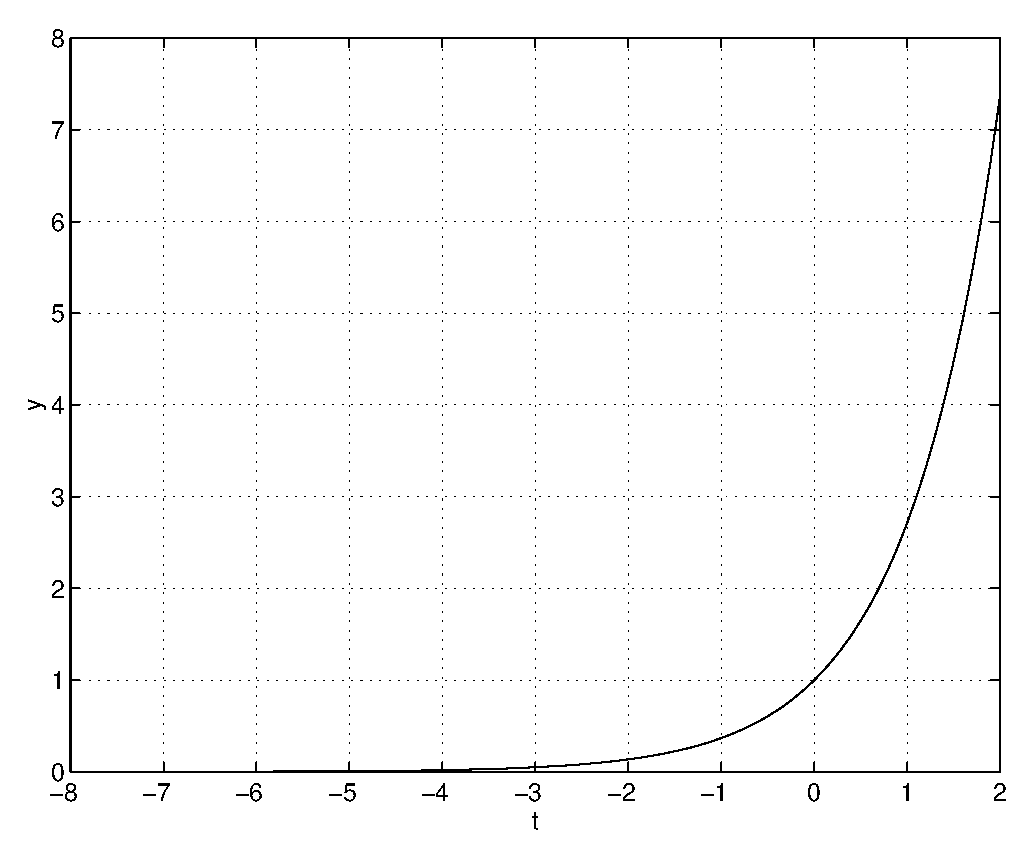
\psfig{file=exfigure/4-4-5a.eps,width=1.8in}
                       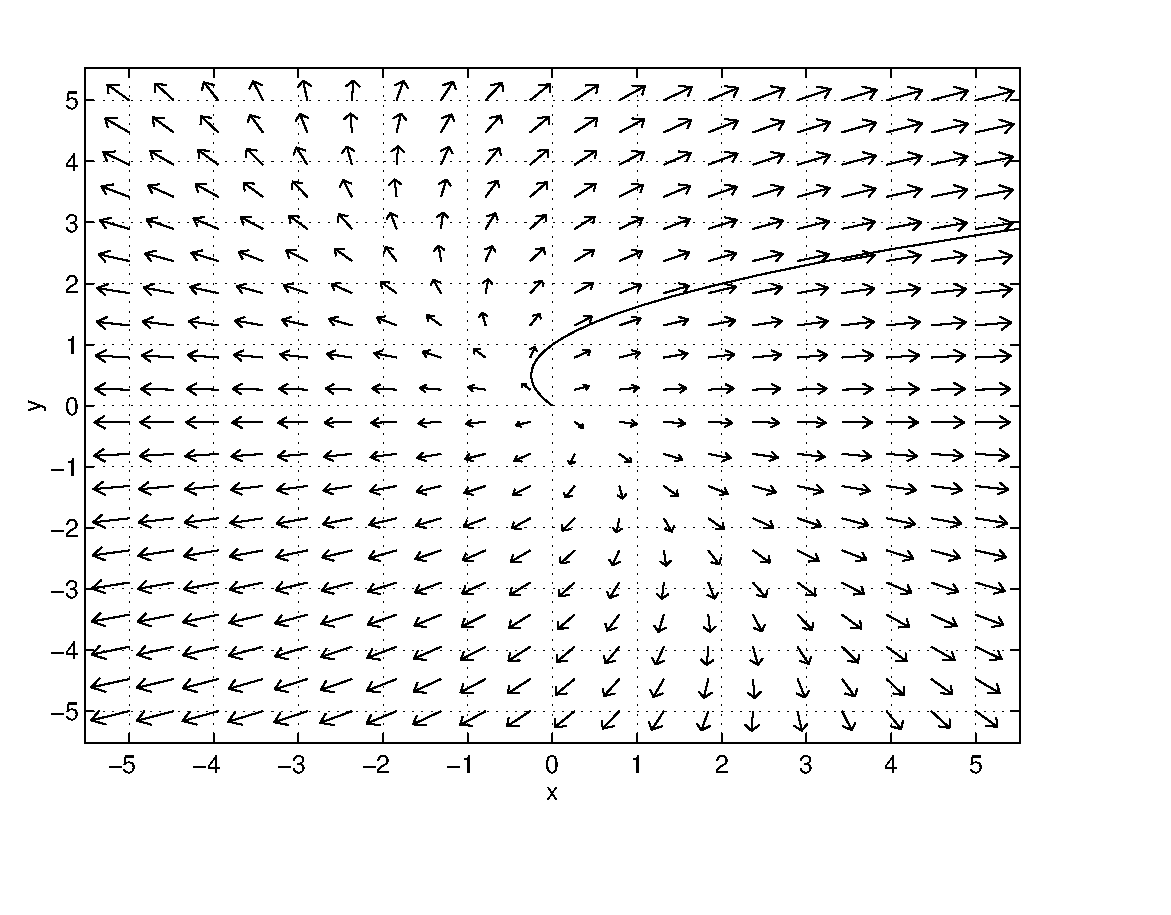
\psfig{file=exfigure/4-4-5b.eps,width=1.8in}
                       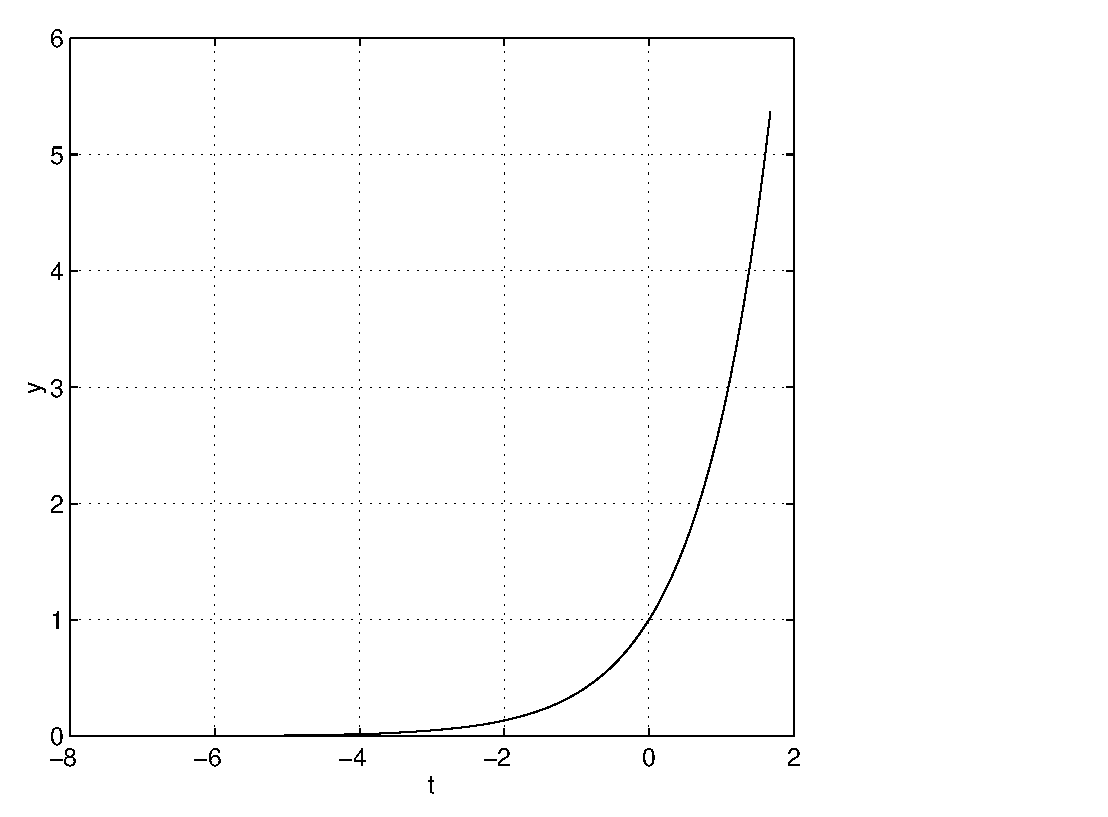
\psfig{file=exfigure/4-4-5c.eps,width=1.8in}}
                \exercapthree{c4.4.5}
\end{figure}



\subsection*{Section~\protect{\ref{S:evchp}} Eigenvalues of $2\times 2$ Matrices}
\rhead{S:evchp}{EIGENVALUES OF $2\times 2$ MATRICES}

\exer{c4.9.2}
\ans The matrix is not invertible when $\lambda = 5$ or $\lambda = -1$.

\soln Corollary~\ref{C:2x2invert} states that a matrix is not invertible
if and only if the determinant is zero; in this case, if
\[
(1 - \lambda)(3 - \lambda) - (2)(4) = \lambda^2 - 4\lambda - 5 = 0.
\]

\newpage
\exer{c6.4.1b} The determinant of the matrix is $23$, the trace is $7$, and
the characteristic polynomial is $p(\lambda)=\lambda^2-7\lambda+23$.

\exer{c6.4.1d} The determinant of the matrix is $0$, the trace is $9$, and
the characteristic polynomial is $p(\lambda)=\lambda^2-9\lambda$.

\exer{c6.4.2b} \ans The eigenvalues of the matrix are
$\lambda_1 = \frac{-3 + \sqrt{17}}{2}$ and $\lambda_2 =
\frac{-3 - \sqrt{17}}{2}$.

\soln The eigenvalues are the roots of the characteristic polynomial, which
is $\lambda^2 + 3\lambda - 2$.

\exer{c6.4.3}
(a) Let
\[
A = \mattwo{a_{11}}{a_{12}}{a_{21}}{a_{22}} \AND
B = \mattwo{b_{11}}{b_{12}}{b_{21}}{b_{22}}
\]

Calculate $\trace(AB)$ and compare to $\trace(BA)$:
\[
\trace(AB) =
\trace\mattwo{a_{11}b_{11} + a_{12}b_{21}}{a_{11}b_{12} + a_{12}b_{22}}
{a_{21}b_{11} + a_{22}b_{21}}{a_{21}b_{12} + a_{22}b_{22}} =
a_{11}b_{11} + a_{12}b_{21} + a_{21}b_{12} + a_{22}b_{22}.
\]

\[
\trace(BA) =
\trace\mattwo{a_{11}b_{11} + a_{21}b_{12}}{a_{12}b_{11} + a_{22}b_{12}}
{a_{11}b_{21} + a_{21}b_{22}}{a_{12}b_{21} + a_{22}b_{22}} =
a_{11}b_{11} + a_{21}b_{12} + a_{12}b_{21} + a_{22}b_{22}.
\]
So, indeed, $\trace(AB) = \trace(BA)$ for $2 \times 2$ matrices
$A$ and $B$.

(b) Let $C = AB$.  Then each element along the main diagonal of $C$ is:
\[
c_{ii} = a_{i1}b_{1i} + \cdots + a_{in}b_{ni} =
\sum_{j = 1}^{n} a_{ij}b_{ji}.
\]
Thus,
\[
\trace(C) = \sum_{i = 1}^{n} \sum_{j = 1}^{n} a_{ij}b_{ji}.
\]
Let $D = BA$.  Then each element along the main diagonal of $D$ is:
\[
d_{ii} = b_{i1}a_{1i} + \cdots + a_{in}b_{ni} =
\sum_{j = 1}^n a_{ij}b_{ji}.
\]
Therefore,
\[
\trace(D) = \sum_{i = 1}^{n} \sum_{j = 1}^{n} b_{ij}a_{ji}
= \sum_{i = 1}^{n} \sum_{j = 1}^{n} a_{ij}b_{ji} = \trace(C).
\]

\exer{c7.8.5b} The mapping has real eigenvalues.  Repeated mapping of any
vector leads to a vector in one of two invariant directions.  These
directions are the eigenvectors.

\newpage
\exer{c7.8.6a} The eigenvectors are $v_1 = (2,1)^t$, with eigenvalue
$\lambda_1 = 4$, and $v_2 = (1,-1)^t$, with eigenvalue $\lambda_2 = -2$.

\exer{c7.8.7} \ans The eigenvalues of $A$ are $\lambda \approx 2.5291 \pm
2.1111i$.

\soln Enter the matrix $A$ into \Matlab and find its eigenvalues by typing
\begin{verbatim}
A = [2.34 -1.43; pi exp(1)];
eig(A)
\end{verbatim}



\subsection*{Section~\protect{\ref{S:IVPR}} Initial Value Problems Revisited}
\rhead{S:IVPR}{INITIAL VALUE PROBLEMS REVISITED}

\exer{c4.10A.1a} \ans The solution to $\dot{X} = CX$ satisfying this
initial condition is
\[
X(t) = 4e^{2t}\vectwo{1}{1} - 3e^t\vectwo{1}{0}
= \cvectwo{4e^{2t} - 3e^t}{4e^{2t}}.
\]

\soln First, find the eigenvalues of $C$, which are the roots of the
characteristic polynomial
\[
p_C(\lambda) = \lambda^2 - \trace(C)\lambda + \det(C) =
\lambda^2 - 3\lambda + 2 = (\lambda - 2)(\lambda - 1).
\]
So the eigenvalues are: $\lambda_1 = 2$ and $\lambda_2 = 1$.
To find the eigenvector associated to each eigenvalue, solve
the equation $(C - \lambda_jI_2)v_j = 0$ for $j = 1$ and $j = 2$.  Solve
\[
\left(\mattwo{1}{1}{0}{2} - \mattwo{2}{0}{0}{2}\right)v_1 =
\mattwo{-1}{1}{0}{0}v_1 = 0
\]
to obtain $v_1 = (1,1)^t$ and solve
\[
\left(\mattwo{1}{1}{0}{2} - \mattwo{1}{0}{0}{1}\right)v_2 =
\mattwo{0}{1}{0}{1}v_2 = 0
\]
to obtain $v_2 = (1,0)^t$.  We can then write the general solution
\[
X(t) = \alpha_1e^{\lambda_1 t}v_1 + \alpha_2e^{\lambda_2 t}v_2
= \alpha_1e^{2t}\vectwo{1}{1} + \alpha_2e^t\vectwo{1}{0}.
\]
From this formula, find $\alpha_1$ and $\alpha_2$ by solving
\[
\vectwo{4}{-3} = X(0) = \alpha_1\vectwo{1}{1} + \alpha_2\vectwo{1}{0} =
\cvectwo{\alpha_1 + \alpha_2}{\alpha_1}.
\]
Solving the linear system
\[
\begin{array}{rrrrr}
\alpha_1 & + & \alpha_2 & = & 4 \\
\alpha_1 & & & = & -3
\end{array}
\]
we obtain $\alpha_1 = 4$ and $\alpha_2 = -3$ and find the
solution to the differential equation.

\exer{c4.10A.1c} \ans The solution to $\dot{X} = CX$ satisfying this
initial condition is
\[
X(t) = \frac{8}{3}e^t\vectwo{1}{2} - \frac{5}{3}e^{-2t}\vectwo{2}{1}
= \frac{1}{3}\cvectwo{8e^t - 10e^{-2t}}{16e^t - 5e^{-2t}}.
\]

\soln First, find the eigenvalues of $C$, which are the roots of the
characteristic polynomial
\[
p_C(\lambda) = \lambda^2 - \trace(C)\lambda + \det(C) =
\lambda^2 + \lambda - 2 = (\lambda - 1)(\lambda + 2).
\]
So the eigenvalues are: $\lambda_1 = 1$ and $\lambda_2 = -2$.
To find the eigenvector associated to each eigenvalue, solve
the equation $(C - \lambda_jI_2)v_j = 0$ for $j = 1$ and $j = 2$.  Solve
\[
\left(\mattwo{-3}{2}{-2}{2} - \mattwo{1}{0}{0}{1}\right)v_1 =
\mattwo{-4}{2}{-2}{1}v_1 = 0
\]
to obtain $v_1 = (1,2)^t$ and solve
\[
\left(\mattwo{-3}{2}{-2}{2} + \mattwo{2}{0}{0}{2}\right)v_2 =
\mattwo{-1}{2}{-2}{4}v_2 = 0
\]
to obtain $v_2 = (2,1)^t$.  We can then write the general solution
\[
X(t) = \alpha_1e^{\lambda_1 t}v_1 + \alpha_2e^{\lambda_2 t}v_2
= \alpha_1e^t\vectwo{1}{2} + \alpha_2e^{-2t}\vectwo{2}{1}.
\]
From this formula, find $\alpha_1$ and $\alpha_2$ by solving
\[
\vectwo{-1}{3} = X(0) = \alpha_1\vectwo{1}{2} + \alpha_2\vectwo{2}{1} =
\cvectwo{\alpha_1 + 2\alpha_2}{2\alpha_1 + \alpha_2}.
\]
Solving the linear system
\[
\begin{array}{rrrrr}
\alpha_1 & + & 2\alpha_2 & = & -1 \\
2\alpha_1 & + & \alpha_2 & = & 3
\end{array}
\]
we obtain $\alpha_1 = \frac{8}{3}$ and $\alpha_2 = -\frac{5}{3}$
and find the solution to the differential equation.

\exer{c4.10A.2} \ans The solution to the differential equation $\dot{X} =
CX$ with the given restrictions is
\[
X(t) = \frac{1}{5}e^{-t}\vectwo{1}{2} + \frac{2}{5}e^{4t}\vectwo{2}{-1}
= \frac{1}{5}\cvectwo{e^{-t} + 4e^{4t}}{2e^{-t} - 2e^{4t}}.
\]

\soln First, find the matrix $C$ using the given information:
First, since $C$ is symmetric, we can write
\[
C = \mattwo{a}{b}{b}{d}.
\]
Then, we are given $\trace(C) = a + d = 3$, so we can rewrite $C$ as
\[
C = \cmattwo{a}{b}{b}{3 - a}.
\]
Since $X(t) = e^{-t}(1,2)^t$ is a solution, $\lambda_1 = -1$
must be an eigenvalue of $C$ with associated eigenvector $v_1 = (1,2)^t$.
Thus $Cv_1 = \lambda_1v_1$, or
\[
\cmattwo{a}{b}{b}{3 - a}\vectwo{1}{2} = \cvectwo{a + 2b}{b + 2(3 - a)}
= \cvectwo{a + 2b}{-2a + b + 6} = \vectwo{-1}{-2}.
\]
This equation yields the linear system
\[
\begin{array}{rrrrr}
a & + & 2b & = & -1 \\
-2a & + & b & = & -8
\end{array}
\]
which we can solve to obtain $a = 3$ and $b = -2$.  So
\[
C = \mattwo{3}{-2}{-2}{0}.
\]
Now, find $\lambda_2$, the other root of
\[
p_C(\lambda) = \lambda^2 - \trace(C) + \det(C) = \lambda^2 - 3\lambda -4
= (\lambda + 1)(\lambda - 4).
\]
Thus, the second eigenvalue of $C$ is $\lambda_2 = 4$, and we can solve
\[
(C - \lambda_2I_2)v_2 = \left(\mattwo{3}{-2}{-2}{0} - \mattwo{4}{0}{0}{4}
\right)v_2 = \mattwo{-1}{-2}{-2}{-4}v_2 = 0
\]
to obtain $v_2 = (2,-1)^t$, the eigenvector associated to $\lambda_2$.
The general solution to $\dot{X} = CX$ is
\[
X(t) = \alpha_1e^{-t}\vectwo{1}{2} + \alpha_2e^{4t}\vectwo{2}{-1}.
\]
Find $\alpha_1$ and $\alpha_2$ by substituting the initial condition $X(0)
= X_0$ into this formula:
\[
\vectwo{1}{0} = X(0) = \alpha_1\vectwo{1}{2} + \alpha_2\vectwo{2}{-1}
= \cvectwo{\alpha_1 + 2\alpha_2}{2\alpha_1 - \alpha_2}.
\]
Thus, $\alpha_1 = \frac{1}{5}$ and $\alpha_2 = \frac{2}{5}$, so we find
the general solution.

\exer{c4.10A.3b} \ans The solution to the differential equation $\dot{X}
= CX$ with the given initial condition is
\[
X(t) \approx 1.0860e^{-1.8035t}\vectwo{-0.9005}{ 0.4348}
- 2.4527e^{4.4835t}\vectwo{-0.8880}{-0.4598}.
\]

\soln In \Matlabp, enter the matrix {\tt C} and the vector {\tt X0}.  Then,
type
\begin{verbatim}
lambda = eig(C)
\end{verbatim}
to obtain the eigenvalues of $C$, which are
$\lambda_1 \approx -1.0835$ and $\lambda_2 \approx 4.4835$.  Find the
eigenvectors $v_1$ and $v_2$ associated to $\lambda_1$ and $\lambda_2$
by typing
\begin{verbatim}
v1 = null(C - lambda(1)*eye(2))
v2 = null(C - lambda(2)*eye(2))
\end{verbatim}
Thus, the general solution is
\[
X(t) = \alpha_1e^{\lambda_1 t}v_1 + \alpha_2e^{\lambda_2 t}v_2
\approx \alpha_1e^{-1.8035t}\vectwo{-0.9005}{ 0.4348} +
\alpha_2e^{4.4835t}\vectwo{-0.8880}{-0.4598}.
\]
The initial condition is
\[
X_0 = X(0) = \alpha_1v_1 + \alpha_2v_2.
\]
We can solve this linear system by creating the matrix $A = (v_1|v_2)$, and
computing $A^{-1}X_0$.  In \Matlabp, type
\begin{verbatim}
A = [v1 v2]
alpha = inv(A)*X0
\end{verbatim}
obtaining $\alpha_1 \approx 1.0860$ and $\alpha_2 \approx -2.4527$.

\exer{c4.10A.4b} \ans $X(0.5) = (1.621,0.291)^t$ and the two methods agree
to three decimal places.

\soln (a) The result of the {\sf pplane5} integration is given in 
Figure~\ref{c4.10A.4b}a. After zooming several times we arrive at
Figure~\ref{c4.10A.4b}b.  By inspection $X(0.5)=(1.621,0.291)$.

(b) (b)  Enter the matrix $C$ into \Matlab by typing
\begin{verbatim}
C = [1.2 2.4; 0.6 -3.5];
\end{verbatim}
Find the eigenvalues and eigenvectors of this matrix by typing {\tt [V,D] = eig(C)}
and obtaining
\begin{verbatim}
V =
    0.9928   -0.4335
    0.1194    0.9011
D =
    1.4887         0
         0   -3.7887
\end{verbatim}
Therefore the general solution to this differential equation is:
\[
X(t) = \alpha e^{1.4887 t}\vectwo{0.9928}{0.1194} +
\beta e^{-3.7887 t}\vectwo{-0.4335}{0.9011}.
\]
It follows that 
\[
X(0) = V \vectwo{\alpha}{\beta}
\]
Therefore,
\[
\vectwo{\alpha}{\beta} = V\inv X_0 = 
\mattwo{0.9928}{-0.4335}{0.1194}{0.9011}\vectwo{0.5}{0.7} = \vectwo{0.7967}{0.6712}
\]
The last calculation is done by typing {\tt coeff = inv(V)*[0.5;0.7]}. 
Therefore, the solution to the initial value problem is:
\[
X(t) = 0.7967e^{1.4887 t}\vectwo{0.9928}{0.1194} +
0.6712e^{-3.7887 t}\vectwo{-0.4335}{0.9011}.
\]
We can evaluate $X(0.5)$ in \Matlab by typing
\begin{verbatim}
X5 = coeff(1)*exp(D(1,1)*0.5)*V(:,1) + coeff(2)*exp(D(2,2)*0.5)*V(:,2)
\end{verbatim}
and obtaining
\begin{verbatim}
X5 =
    1.6213
    0.2912
\end{verbatim}

(c)  The two answers agree to three decimal places.

\begin{figure}[htb]
                       \centerline{%
                       \psfig{file=exfigure/4-9-9a.eps,width=2.75in}
                       \psfig{file=exfigure/4-9-9b.eps,width=2.75in}}
                \exercaptwo{c4.10A.4b}
\end{figure}



\subsection*{Section~\protect{\ref{S:TransitionApplied}} Markov Chains}
\rhead{S:TransitionApplied}{MARKOV CHAINS}

\exer{c4.10.1}
Let
\[ P = \left(\begin{array}{ccc} p_{11} & \cdots & p_{1n} \\
\vdots & \ddots & \vdots \\ p_{n1} & \cdots & p_{nn}
\end{array}\right). \]
Then,
\[ Pw = \left(\begin{array}{ccc} p_{11} & \cdots & p_{1n} \\
\vdots & \ddots & \vdots \\ p_{n1} & \cdots & p_{nn}
\end{array}\right) \cvecthree{1}{\vdots}{1} = 
\cvecthree{p_{11} + \cdots + p_{1n}}{\vdots}{p_{n1} + \cdots +
p_{nn}} = \cvecthree{1}{\vdots}{1} \]
since the sum of the entries in each row of a Markov matrix is $1$.

\exer{c4.10.2b} Matrix $Q$ is not a Markov matrix, since there is no
positive integer $k$ for which $Q^k(2,1) > 0$.

\exer{c4.10.3}
Let $P$ be the transition matrix associated with Figure~\ref{F:Mchain}.
Then,
\[ P = \left(\begin{array}{rrrrr}
\frac{1}{3} & 0 & \frac{1}{3} & \frac{1}{3} & 0 \\
\frac{1}{3} & \frac{1}{3} & \frac{1}{3} & 0 & 0 \\
0 & 0 & \frac{1}{2} & \frac{1}{2} & 0 \\
0 & 0 & 0 & \frac{1}{2} & \frac{1}{2} \\
\frac{1}{4} & \frac{1}{4} & 0 & \frac{1}{4} & \frac{1}{4}
\end{array}\right). \]

\exer{c4.10.5}
(a) \ans Let $D =${\tt PDOG} be the transition matrix for this Markov chain:
\[
D = \left(\begin{array}{rrrr} 0 & \frac{1}{3} & \frac{1}{3} &
\frac{1}{3} \\ 1 & 0 & 0 & 0 \\ 0 & 0 & 0 & 1 \\
0 & \frac{1}{2} & \frac{1}{2} & 0 \end{array}\right).
\]

\soln All entries of $D$ are nonnegative and the entries of each row of
$D$ sum to $1$.  The \Matlab command {\tt D\^{}5} verifies that all
entries of the matrix $D^5$ are positive.  Therefore,
Definition~\ref{D:Markov} is valid for $D$.

(b) The probability that a dog starting in room 2 will end up in room
3 after 5 steps is element $(2,3)$ of the matrix $D^5$, or
$\frac{7}{36}$.

(c) \ans The probability that a dog starting in room 3 will end up in room
1 after 4 steps is 0.

\soln The only way a dog in room 3 can get to room 1
is by going from room 3 to room 4, then to room 2, then to room 1, which
takes three steps.  The dog must then leave room 1 on the fourth step,
and there is no other combination of steps by which the dog could go to
room 1 in four steps.

(d) \ans After a large number of steps, there will be approximately $23$
dogs in each of rooms 1, 2, and 3, and $31$ dogs in room 4.

\soln Using \Matlab, evaluate $D^k$ for large values of $k$.

\newpage
\exer{c4.10.7}
(a) The probability that an individual at site 2 will move to site 5 in
three steps is $11.62\%$, that is, element $(2,5)$ of $P^3$.

(b) The probability that an individual at site 4 will move to site 1 in
seven steps is $14.07\%$, that is, element $(4,1)$ of $P^7$.

(c) After four steps, the distribution will be
\[ (P^t)^4\left(\begin{array}{r} 20 \\ 20 \\ 20 \\ 20 \\ 20
\end{array}\right) = \left(\begin{array}{r} 14.1466 \\ 22.1620 \\
21.2874 \\ 30.0624 \\ 12.3417 \end{array}\right). \]

(d) \ans Let $V$ be an eigenvector of $P^t$ with eigenvalue 1.
\[
V = \left(\begin{array}{r} 0.1408 \\ 0.2195 \\ 0.2154 \\ 0.3032
\\ 0.1211 \end{array}\right).
\]

\soln \Matlab can be used to verify that $P^tV = V$.  To find this
eigenvector, evaluate the matrix $(P^t)^k$ for large values of $k$.
The vector $V$ is any column of this matrix.

\exer{c4.10.9}
\ans The probability that the man will get wet going to work is $1.53\%$.

\soln Create the $4 \times 4$ matrices $P$ (the transition matrix between
morning and afternoon) and $Q$ (the transition matrix between afternoon
and the next morning), then multiply to obtain \begin{verbatim}
R =
    0.7000    0.3000         0         0
    0.1400    0.6200    0.2400         0
         0    0.1400    0.6200    0.2400
         0         0    0.1400    0.8600
\end{verbatim}
Find the eigenvector $V$ of $R$.  The first element of $V$ is $0.0763$,
the probability that there will be no umbrella in the house on a given
morning.  Multiply this by the probability that it will rain in the
morning to obtain the solution.



\end{document}
